%% Version 4.3.2, 25 August 2014
%
%%%%%%%%%%%%%%%%%%%%%%%%%%%%%%%%%%%%%%%%%%%%%%%%%%%%%%%%%%%%%%%%%%%%%%
% Template.tex --  LaTeX-based template for submissions to the 
% American Meteorological Society
%
% Template developed by Amy Hendrickson, 2013, TeXnology Inc., 
% amyh@texnology.com, http://www.texnology.com
% following earlier work by Brian Papa, American Meteorological Society
%
% Email questions to latex@ametsoc.org.
%
%%%%%%%%%%%%%%%%%%%%%%%%%%%%%%%%%%%%%%%%%%%%%%%%%%%%%%%%%%%%%%%%%%%%%
% PREAMBLE
%%%%%%%%%%%%%%%%%%%%%%%%%%%%%%%%%%%%%%%%%%%%%%%%%%%%%%%%%%%%%%%%%%%%%

%% Start with one of the following:
% DOUBLE-SPACED VERSION FOR SUBMISSION TO THE AMS
\documentclass{ametsoc}

% TWO-COLUMN JOURNAL PAGE LAYOUT---FOR AUTHOR USE ONLY
% \documentclass[twocol]{ametsoc}

%%%%%%%%%%%%%%%%%%%%%%%%%%%%%%%%
%%% To be entered only if twocol option is used

\journal{jas}

%  Please choose a journal abbreviation to use above from the following list:
% 
%   jamc     (Journal of Applied Meteorology and Climatology)
%   jtech     (Journal of Atmospheric and Oceanic Technology)
%   jhm      (Journal of Hydrometeorology)
%   jpo     (Journal of Physical Oceanography)
%   jas      (Journal of Atmospheric Sciences)	
%   jcli      (Journal of Climate)
%   mwr      (Monthly Weather Review)
%   wcas      (Weather, Climate, and Society)
%   waf       (Weather and Forecasting)
%   bams (Bulletin of the American Meteorological Society)
%   ei    (Earth Interactions)

%%%%%%%%%%%%%%%%%%%%%%%%%%%%%%%%
%Citations should be of the form ``author year''  not ``author, year''
\bibpunct{(}{)}{;}{a}{}{,}

%%%%%%%%%%%%%%%%%%%%%%%%%%%%%%%%

%%% To be entered by author:

%% May use \\ to break lines in title:

\title{Tropopause Evolution in a Rapidly Intensifying Tropical Cyclone: A Static Stability Budget Analysis in an Idealized, Axisymmetric Framework}

%%% Enter authors' names, as you see in this example:
%%% Use \correspondingauthor{} and \thanks{Current Affiliation:...}
%%% immediately following the appropriate author.
%%%
%%% Note that the \correspondingauthor{} command is NECESSARY.
%%% The \thanks{} commands are OPTIONAL.

    %\authors{Author One\correspondingauthor{Author One, 
    % American Meteorological Society, 
    % 45 Beacon St., Boston, MA 02108.}
% and Author Two\thanks{Current affiliation: American Meteorological Society, 
    % 45 Beacon St., Boston, MA 02108.}}

\authors{Patrick Duran\correspondingauthor{Department of Atmospheric and Environmental Sciences, University at Albany, State University of New York, 1400 Washington Avenue, Albany, NY.} and John Molinari}

%% Follow this form:
    % \affiliation{American Meteorological Society, 
    % Boston, Massachusetts.}

\affiliation{University at Albany, State University of New York,
Albany, NY}

%% Follow this form:
    %\email{latex@ametsoc.org}

\email{pduran2008@gmail.com}

%% If appropriate, add additional authors, different affiliations:
    %\extraauthor{Extra Author}
    %\extraaffil{Affiliation, City, State/Province, Country}

%\extraauthor{}
%\extraaffil{}

%% May repeat for a additional authors/affiliations:

%\extraauthor{}
%\extraaffil{}

%%%%%%%%%%%%%%%%%%%%%%%%%%%%%%%%%%%%%%%%%%%%%%%%%%%%%%%%%%%%%%%%%%%%%
% ABSTRACT
%
% Enter your abstract here
% Abstracts should not exceed 250 words in length!
%
% For BAMS authors only: If your article requires a Capsule Summary, please place the capsule text at the end of your abstract
% and identify it as the capsule. Example: This is the end of the abstract. (Capsule Summary) This is the capsule summary. 

\abstract{Large changes in tropopause-layer static stability are observed during the rapid intensification (RI) of an idealized, axisymmetric tropical cyclone (TC).
Over the eye, static stability near the tropopause decreases and the cold-point tropopause height rises by up to 4 km at the storm center.
Outside of the eye, static stability increases considerably just above the cold-point tropopause, and the tropopause remains near its initial level.\\
\indent A budget analysis reveals that advection contributes to the static stability tendencies at all times throughout the upper troposphere and lower stratosphere.
Advection is particularly important within the eye, where it acts to destabilize the layer near and above the cold-point tropopause.
Outside of the eye, a radial-vertical circulation develops during RI, with strong outflow below the tropopause and weak inflow above.
Vertical wind shear above and below the upper-tropospheric outflow maximum induces turbulence, which provides forcing for both destabilization and stabilization in the tropopause layer.
Meanwhile, as organized convection reaches the tropopause, radiative heating tendencies at the top of the cirrus canopy generally act to destabilize the upper troposphere and stabilize the lower stratosphere.
Turbulent mixing and radiative heating combine to play an important role in the development of the strong stable layer immediately above the cold-point tropopause during RI.
The results suggest that turbulence and radiation, alongside advection, play fundamental roles in the upper-level static stability evolution of TCs.}
%The conclusions are robust to changes in the initial thermodynamic profile and prescribed vertical mixing length within a reasonable range of values.}

\begin{document}

%% Necessary!
\maketitle


%%%%%%%%%%%%%%%%%%%%%%%%%%%%%%%%%%%%%%%%%%%%%%%%%%%%%%%%%%%%%%%%%%%%%
% MAIN BODY OF PAPER
%%%%%%%%%%%%%%%%%%%%%%%%%%%%%%%%%%%%%%%%%%%%%%%%%%%%%%%%%%%%%%%%%%%%%
%

%% In all cases, if there is only one entry of this type within
%% the higher level heading, use the star form: 
%%
 \section{Introduction}

%Perhaps introduce upper-tropospheric static stability and its relationship to the diurnal cycle before going into Patricia? Include references to Dunion, Navarro, and O'Neill here.
%More recently, \cite{Dunionetal2014} documented a periodic oscillation of infrared brightness temperature in hurricanes, which they call the "TC diurnal pulse."
%There will be a whole bunch of papers cited here...
%At some point (probably in the Discussion) mention the possible importance of static stability asymmetries, in the context of the Dunion diurnal pulse 

After undergoing a remarkably rapid intensification (RI), Hurricane Patricia (2015) set a new record as the strongest tropical cyclone (TC) ever observed in the Western Hemisphere (\citeauthor{Kimberlainetal2016} \citeyear{Kimberlainetal2016}; \citeauthor{Rogersetal2017} \citeyear{Rogersetal2017}).
High-altitude dropsonde observations taken during the Tropical Cyclone Intensity (TCI) experiment captured this RI in unprecedented detail \citep{DoyleTCI}.
These observations revealed dramatic changes in the structure of the cold-point tropopause and upper-level static stability as the storm intensified \citep{DuranMolinari2018}.

At tropical storm intensity, shortly before RI commenced, a strong inversion layer existed just above Patricia's cold-point tropopause, which was located near 17.2 km.
During the first half of the RI period, this inversion layer weakened throughout Patricia's inner core, with the weakening most pronounced over the developing eye.
By the time the storm reached its maximum intensity, the inversion layer over the eye had disappeared almost completely, which was accompanied by an increase in the tropopause height to a level at or above the highest-available dropsonde data point (18.3 km) at two locations.
Meanwhile over the eyewall region, the static stability re-strengthened and the tropopause was limited to a level at or below 17.5 km.
The mechanisms that led to these changes in upper-level static stability and tropopause height are the subject of the current paper.

Despite the importance of tropopause-layer thermodynamics in theoretical models of hurricanes (\citeauthor{EmanuelRotunno2011} \citeyear{EmanuelRotunno2011}; \citeauthor{Emanuel2012} \citeyear{Emanuel2012}), few papers have examined the upper-tropospheric evolution of TCs.
\cite{KomaromiDoyle2017} found that stronger TCs tended to have a higher and warmer tropopause over their inner core than weaker TCs.
Their results are consistent with the evolution observed over the inner core of Hurricane Patricia, in which the tropopause height increased and the tropopause temperature warmed throughout RI \citep{DuranMolinari2018}.

Idealized simulations of a TC analyzed by \cite{OhnoSatoh2015} suggested that the development of an upper-level warm core near the TC storm center acted to decrease the static stability near the tropopause (compare their Figs. 9,10).
Although the mechanisms that drive this static stability evolution have not been examined explicitly, \cite{SternZhang2013} described the development of the TC warm core using a potential temperature ($\theta$) budget analysis.
They found that radial and vertical advection both played important roles in warm core development throughout RI, and subgrid-scale diffusion became particularly important during the later stage of RI.
To our knowledge, the only paper that has examined explicitly the static stability evolution in a modeled TC is \cite{Kepertetal2016}, but their analysis was limited to the boundary layer.
The analysis herein is based upon that of \cite{SternZhang2013}, except using a static stability budget similar to that of \cite{Kepertetal2016}, with a focus on the upper troposphere and lower stratosphere.

 \section{Model Setup}

The numerical simulations were performed using version 19.4 of Cloud Model 1 (CM1) described in \cite{BryanRotunno2009}.
The equations of motion were integrated on a 3000-km-wide, 30-km-deep axisymmetric grid with 1-km horizontal and 250-m vertical grid spacing.
The computations were performed on an \textit{f}-plane at 15\textdegree{N} latitude, over a sea surface with constant temperature of 30.5\textdegree C, which matches that observed near Hurricane Patricia (2015; \citeauthor{Kimberlainetal2016} \citeyear{Kimberlainetal2016}).
Horizontal turbulence was parameterized using the Smagorinsky scheme described in \citeauthor{BryanRotunno2009} (\citeyear{BryanRotunno2009}, pg. 1773), with a prescribed mixing length that varied linearly from 100 m at a surface pressure of 1015 hPa to 1000 m at a surface pressure of 900 hPa.
This formulation allows for realistically-large horizontal mixing lengths near the hurricane's inner core, consistent with the results of \cite{Bryan2012}, while not over-representing horizontal turbulence in convection at outer radii.
Vertical turbulence was parameterized using the formulation of \citeauthor{MarkowskiBryan2016} (\citeyear{MarkowskiBryan2016}, their Eq. 6), using an asymptotic vertical mixing length of 100 m and a vertically implicit Crank-Nicholson scheme.
A Rayleigh damping layer was applied outside of the 2900-km radius and above the 25-km level to prevent spurious gravity wave reflection at the model boundaries.
Microphysical processes were parameterized using the \cite{Thompson} microphysics scheme and radiative heating tendencies were computed every two minutes using the Rapid Radiative Transfer Model for GCMs (RRTMG) longwave and shortwave schemes \citep{Iacono}.
The initial temperature and humidity field was horizontally homogeneous and determined by averaging all Climate Forecast System Reanalysis (CFSR) grid points within 100 km of Patricia's center of circulation at 18 UTC 21 October 2015.
%A horizontally-homogeneous temperature and humidity field was initialized with a mean sounding computed using all dropsondes deployed during the TCI flight conducted within and around Tropical Storm Patricia on 21 October, 2015 (see \citeauthor{DoyleTCI} \citeyear{DoyleTCI} for details.)
%Above 19 km, where few TCI observations were available, the temperature profile was taken from the Climate Forecast System Reanalysis (CFSR) grid point nearest Patricia's storm center, valid at 18 UTC 21 October, 2015.
%Since relative humidity measurements were unreliable at temperatures below -40\textdegree C \citep{BellTCI}, relative humidity was set equal to 50\% above 11.5 km (the level above which temperature dropped below -40\textdegree C).
The vortex described in \citeauthor{RotunnoEmanuel} (\citeyear{RotunnoEmanuel}, their Eq. 37) was used to initialize the wind field, setting all parameters equal to the values used therein.

Although hurricanes simulated in an axisymmetric framework tend to be more intense than those observed in nature, the intensity evolution of this simulation matches reasonably well with that observed in Hurricane Patricia.
After an initial spin-up period of about 20 hours, the modeled storm (Fig.\ref{fig:vmax+pmin}, blue lines) began an RI period that lasted approximately 30 hours.
After this RI, the storm continued to intensify more slowly until the maximum 10-m wind speed reached 89 m s\textsuperscript{-1} and the minimum sea-level pressure reached its minimum of 846 mb, 81 hours into the simulation.
Hurricane Patricia (red stars) exhibited a similar intensity evolution, with an RI period leading to a maximum 10-m wind speed of 95 m s\textsuperscript{-1} and a minimum sea-level pressure of 872 hPa.
Despite the limitations of the axisymmetric framework, the extraordinary intensity of Hurricane Patricia and the rapidity of its intensification makes Patricia a particularly good candidate for axisymmetric analysis.

 \section{Budget Computation}

The static stability can be expressed as the squared Brunt V{\"a}is{\"a}l{\"a} frequency:
   \begin{equation} \label{eq:n2moist}
   N_m^2 = \frac{g}{T}\left(\frac{\partial T}{\partial z}+\Gamma_m\right)\left(1+\frac{T}{R_d/R_v+q_s}\frac{\partial q_s}{\partial T}\right)-\frac{g}{1+q_t}\frac{\partial q_t}{\partial z},
   \end{equation}
where $g$ is gravitational acceleration, $T$ is temperature, $R_d$ and $R_v$ are the gas constants of dry air and water vapor, respectively, $q_s$ is the saturation mixing ratio, $q_t$ is the total condensate mixing ratio, and $\Gamma_m$ is the moist-adiabatic lapse rate:
   \begin{equation} \label{eq:gamma_m}
   \Gamma_m = g(1+q_t)\left(\frac{1+L_vq_s/R_dT}{c_p_m +L_v\partial q_s/\partial T}\right),
   \end {equation}
where $L_v$ is the latent heat of vaporization and $c_{pm}$ is the specific heat of moist air at constant pressure.
In the tropopause layer, $q_s$, ${\partial q_s}/{\partial T}$, and ${\partial q_t}/{\partial z}$ approach zero. In this limiting case, Eq. \ref{eq:n2moist} reduces to:
   \begin{equation} \label{eq:n2dry}
   N^2 = \frac{g}{\theta}\frac{\partial \theta}{\partial z},
   \end{equation}
where $\theta$ is the potential temperature.

To compute $N^2$, CM1 uses Eq.\ref{eq:n2moist} in saturated environments and Eq. \ref{eq:n2dry} in sub-saturated environments. For simplicity, however, only Eq. \ref{eq:n2dry} will be employed for the budget computations herein\footnote{The validity of this approximation will be substantiated later in this section.}.

Taking the time derivative of Eq. \ref{eq:n2dry} yields the static stability tendency:
   \begin{equation} \label{eq:dn2dt}
   \frac{\partial N^2}{\partial t} = \frac{g}{\theta}\frac{\partial}{\partial z}\frac{\partial \theta}{\partial t}-\frac{g}{\theta^2}\frac{\partial \theta}{\partial z}\frac{\partial \theta}{\partial t},
   \end{equation}
where the potential temperature tendency, $\partial \theta/\partial t$, can be written:
   \begin{equation} \label{eq:dthetadt}
   \frac{\partial \theta}{\partial t} = HADV+VADV+HTURB+VTURB+MP+RAD+DISS 
   \end{equation}
Each term on the right-hand side of Eq. \ref{eq:dthetadt} represents a $\theta$ budget variable, each of which is output directly by the model every minute.
HADV and VADV are the radial and vertical advective tendencies\footnote{These terms include the tendencies due to the diffusion that is implicit in the fifth-order advection scheme.}, HTURB and VTURB are the radial and vertical tendencies from the turbulence parameterization, MP is the tendency from the microphysics scheme, RAD is the tendency from the radiation scheme, and DISS is the tendency due to turbulent dissipation.
This equation neglects Rayleigh damping, since this term is zero everywhere below 25 km, and the analysis domain does not extend to that level.
Each term in Eq. \ref{eq:dthetadt} is substituted for ${\partial \theta}/{\partial t}$ in Eq. \ref{eq:dn2dt}, yielding the contribution of each budget term to the static stability tendency.
These terms are summed, yielding an instantaneous "budget change" in $N^2$ every minute.
The budget changes are then averaged over 24-hour periods and compared to the total model change in $N^2$ over that same time period, i.e.:
   \begin{equation} \label{eq:budgetchange}
   \Delta N^2_{budget} = \frac{1}{\delta t}\sum_{t=t_0}^{t_0+\delta t} \left.\frac{\partial N^2}{\partial t}\right\vert_t
   \end{equation}
   \begin{equation} \label{eq:modelchange}
   \Delta N^2_{model} = N^2_{t_0+\delta t}-N^2_{t_0}
   \end{equation}
   \begin{equation} \label{eq:residual}
   Residual = \Delta N^2_{model}-\Delta N^2_{budget}
   \end{equation}
where $t_0$ is an initial time and $\delta t$ is 24 hours.

Eqs. \ref{eq:budgetchange}-\ref{eq:residual} are plotted for four consecutive 24-hour periods in Fig. \ref{fig:mod+bud+res}.
For this and all subsequent radial-vertical cross sections, a 1-2-1 smoother is applied once in the radial direction to eliminate $2\Delta r$ noise that appears in some of the raw model output and calculated fields.
The left column of Fig.~\ref{fig:mod+bud+res} depicts the model changes (Eq. \ref{eq:modelchange}), the center column depicts the budget changes (Eq. \ref{eq:budgetchange}), and the right column depicts the residuals (Eq. \ref{eq:residual}).
In every 24-hour period, the budget changes are nearly identical to the model changes, which is reflected in the near-zero residuals in the right column.
This indicates that the budget accurately represents the model variability, which implies that the neglect of moisture in the budget computation introduces negligible error within the anaysis domain\footnote{This is not the case in the lower- and mid-troposphere, where the residual actually exceeds the budget variability in many places, likely due to the neglect of moisture; thus we limit this analysis to the upper troposphere and lower stratosphere.}.

In the tropopause layer, some of the budget terms are small enough to be ignored.
To determine which of the budget terms are most important, a time series of the contribution of each of the budget terms in Eq. \ref{eq:dthetadt} to the tropopause-layer static stability tendency is plotted in Fig. \ref{fig:avgbudterms}.
For this figure, each of the budget terms is computed using the method described in Section 3, except with 1-hour averaging intervals instead of 24-hour intervals.
The absolute values of these tendencies are then averaged over a radius-height domain surrounding the tropopause and plotted as a time series\footnote{It will be seeen in subsequent figures that each of the terms contributes both positively and negatively to the $N^2$ tendency within the analysis domain. 
Thus, taking an average over the domain tends to wash out the positive and negative contributions.
To circumvent this problem, the absolute value of each of the terms is averaged.}. 
Advection (Fig.~\ref{fig:avgbudterms}, red line) plays an important role in the mean tropopause-layer static stability tendency at all times, and vertical turbulence (Fig.~\ref{fig:avgbudterms}, blue line) and radiation (Fig.~\ref{fig:avgbudterms}, dark green line) also contribute significantly. %both become important after 48 hours.
Although the contribution from horizontal turbulence (Fig.~\ref{fig:avgbudterms}, purple line) becomes more important after 48 hours, it is confined to a very small region immediately surrounding the eyewall tangential velocity maximum (not shown), and is negligible throughout the rest of the tropopause layer.
The remaining two processes - microphysics and dissipative heating (Fig.~\ref{fig:avgbudterms}, orange and light green lines, respectively) - lie atop one another near zero.
Although the latent heating term can be quite large in the eyewall region, it is negligible everywhere outside of the eyewall, as are the effects of dissipative heating.
These time series indicate that, at all times, three budget terms dominate the tropopause-layer static stability tendency: advection, vertical turbulence, and radiation.
Variations in the magnitude and spatial structure of these terms drive the static stability changes depicted in Fig.~\ref{fig:mod+bud+res}; subsequent sections will focus on these variations and what causes them.

 \section{Results}

 \subsection{Static stability evolution}

The average $N^2$ over the first day of the simulation (Fig.~\ref{fig:n2-24hr-avgs}a) indicates the presence of a weak static stability maximum just above the cold-point tropopause.
Over the subsequent 24 hours, during the RI period, the static stability within and above this layer decreased near the storm center (Fig.~\ref{fig:n2-24hr-avgs}b).
This decreasing $N^2$ corresponded to an increase in the tropopause height within the developing eye, maximized at the storm center.
Outside of the eye, meanwhile, the tropopause height decresed over the eyewall region (25-60-km radius) and increased only slightly outside of the 60-km radius.
In this outer region, the $N^2$ maximum just above the tropopause strengthened during RI.
These trends continued as the storm's intensity leveled off in the 48-72-hour period (Fig.~\ref{fig:n2-24hr-avgs}c).
The tropopause height increased to nearly 21 km at the storm center and sloped sharply downward to 16.3 km on the inner edge of the eyewall, near the 30 km radius.
Static stability outside of the eye, meanwhile, continued to increase just above the cold-point tropopause.
This $N^2$ evolution closely follows that observed in Hurricane Patricia (2015; \citeauthor{DuranMolinari2018} \citeyear{DuranMolinari2018}).
The mechanisms that led to these static stability changes will be investigated in the subsequent sections.

 \subsection{Static stability budget analysis}

\paragraph{0-24 hours}
The weakening of the lower-stratospheric static stability maximum during the initial spin-up period is reflected in the total $N^2$ budget change over this time (Fig.~\ref{fig:stab-00-24}a).
The 17-18-km layer was characterized by decreasing $N^2$ (purple shading), maximizing at the storm center.
The layer immediately below the tropopause, meanwhile, saw strengthening $N^2$ during this time period.
Although these tendencies extended out to the 200-km radius, they were particularly pronounced at innermost radii.
A comparison of the contributions of advection (Fig.~\ref{fig:stab-00-24}b), vertical turbulence (Fig.~\ref{fig:stab-00-24}c), and radiation (Fig.~\ref{fig:stab-00-24}d) reveals that advection was primarily responsible for the change in static stability during this period.
Although vertical turbulence acted in opposition to advection (i.e. it acted to stabilize regions that advection acted to destabilize), the magnitude of the advective tendencies was larger, particularly at the innermost radii.
The sum of advection and vertical turbulence (Fig.~\ref{fig:stab-00-24}e) almost exactly replicated the static stability tendencies above 17 km.
Radiative tendencies. meanwhile, (Fig.~\ref{fig:stab-00-24}d) acted to destabilize the layer below about 16 km and stabilize the layer between 16 and 17 km.
The sum of advection, vertical turbulence, and radiation (Fig.~\ref{fig:stab-00-24}f) reproduces the total change in $N^2$ almost exactly.

\paragraph{24-48 hours}
During the RI period, $N^2$ within the eye generally decreased above 16 km and increased below (Fig.~\ref{fig:stab-24-48}a).
These tendencies at the innermost radii were driven almost entirely by advection (Fig.~\ref{fig:stab-24-48}b); vertical turbulence (Fig.~\ref{fig:stab-24-48}c) and radiation (Fig.~\ref{fig:stab-24-48}d) contributed negligibly to the static stability tendencies in this region.

Outside of the eye, the $N^2$ evolution exhibited alternating layers of positive and negative tendencies.
Near and above 18 km existed an upward-sloping region of decreasing $N^2$ that extended out to the 180-km radius.
In this region, neither vertical turbulence nor radiation exhibited negative $N^2$ tendencies; advection was the only forcing for destabilization.
Immediately below this layer was a region of increasing $N^2$, which sloped upward from 17 km near the 30-km radius to just below 18 km outside of the 100-km radius.
Advection and vertical turbulence both contributed to this positive $N^2$ tendency, with advection playing an important role below about 17.5 km and and turbulence playing an important role above.
The sum of advection and turbulence (Fig.~\ref{fig:stab-24-48}e) reveals two discontiguous regions of increasing $N^2$ in the 17-18-km layer rather than one contiguous region.
The addition of radiation to these two terms, however, (Fig.~\ref{fig:stab-24-48}f) provides the link between these two regions, indicating that radiation also plays a role in strengthening the stable layer just above the tropopause.
In the 16-17-km layer, a horizontally-extensive layer of decreasing $N^2$ also was forced by a combination of advection, vertical turbulence, and radiation.
The sum of advection and vertical turbulence accounts for only a portion of the decreasing $N^2$ in this layer, and actually indicates forcing for stabilization near the 50-km radius and outside of the 130-km radius.
Radiative tendencies overcome this forcing for stabilization in both of these regions to produce the radially-extensive region of destabilization observed just below the tropopause.

The sum of advection, vertical turbulence, and radiation (Fig. \ref{fig:stab-24-48}f) once again closely follows the observed $N^2$ variability, except in portions of the eyewall where the neglect of latent heating and horizontal turbulence introduces some differences.

\paragraph{48-72 hours}
After the storm's maximum wind speed leveled off near 80 m s\textsuperscript{-1}, the magnitude of the static stability tendencies within the eye decreased to near zero (Fig.~\ref{fig:stab-48-72}a).

Outside of the eye, however, $N^2$ continued to increase just above the tropopause and decrease just below.
The sum of advection and vertical turbulence (Fig.~\ref{fig:stab-48-72}e) indicates that the increase of $N^2$ observed in the 17-18-km layer and inside of the 80-km radius cannot be attributed to these processes, since the sum of these two terms provided forcing for destabilization.
Instead, radiation (Fig.~\ref{fig:stab-48-72}d), provided the forcing for stabilization in this region.
Outside of the 80-km radius, both advection (Fig.~\ref{fig:stab-48-72}b) and vertical turbulence (Fig.~\ref{fig:stab-48-72}c) provided forcing for stabilization near the 18-km level.
The sum of the two terms indicates increasing $N^2$ near the 18-km level everywhere outside of the 80-km radius, but this stabilization is slightly weaker in the 90-120-km radial band than the observed value.
The addition of radiation (Fig.~\ref{fig:stab-48-72}f) provides the extra forcing for stabilization required to account for the observed increase in $N^2$.
Outside of the 120-km radius, the region of radiative forcing for stabilization slopes downward, and the increase in $N^2$ observed near 18 km can be explained entirely by a combination of advection and vertical turbulence.
The layer of decreasing $N^2$ observed near 17 km was forced primarily by vertical turbulence and radiation.
Within most of this region, advection provided strong forcing for stabilization, but this forcing was outweighed by the negative $N^2$ tendencies induced by a combination of vertical turbulence and radiation.

  \section{Discussion}

  \subsection{The role of advection}

Advection played an important role in the tropopause-layer $N^2$ evolution at all stages of intensification, but for brevity, this section will focus only on the RI (24-48-hour) period.
To investigate the advective processes more closely, the individual contributions of horizontal and vertical advection during the RI period are shown in Fig. \ref{fig:adv-24-48}, along with the corresponding time-mean radial and vertical velocities and $\theta$.
The $N^2$ tendencies due to the two advective components (Fig. \ref{fig:adv-24-48}a,b) exhibit strong cancellation, consistent with flow that is nearly isentropic.
There are, however, many regions in which flow crosses $\theta$ surfaces; this flow accounts for all non-zero $N^2$ tendencies due to advection previously seen in Fig. \ref{fig:stab-24-48}b.

%The eye was characterized by stabilization below 16 km and destabilization in the 16-17-km and 18-19-km layers.
%Comparing Fig. \ref{fig:stab-24-48}b to \ref{fig:adv-24-48}a,b reveals that the stabilization below 16 km in the eye was forced by vertical advection, as was the region of destabilization in the 18-19-km layer.
%Meanwhile, the destabilization that occurred in the 16-17-km layer was forced by a combination and radial and vertial advection.

%Outside of the eye, the layer below about 15.5 km was dominated by stabilization.
%Outside of the 50-km radius, horizontal advection provided the forcing for this stabilization, while inside of the 50-km radius, vertical advection was responsible.
%Above this layer existed a layer of destabilization near the 16-km level, which was forced by horizontal advection.


Some insight can be gained by considering the time tendency of the vertical $\theta$ gradient due to advection:
   \begin{equation} \label{eq:advtend}
   \left(\frac{\partial}{\partial t}\frac{\partial \theta}{\partial z}\right)_{adv} = -u\frac{\partial}{\partial r}\frac{\partial \theta}{\partial z}-w\frac{\partial}{\partial z}\frac{\partial \theta}{\partial z}-\frac{\partial u}{\partial z}\frac{\partial \theta}{\partial r}-\frac{\partial w}{\partial z}\frac{\partial \theta}{\partial z}.
   \end{equation}

The first two terms on the right-hand side of Eq. \ref{eq:advtend} represent advection of static stability by the radial and vertical wind, respectively.
These terms cannot create a maximum or a minimum; they only act to rearrange the static stability field.
%Since the goal of this analysis is to understand the processes responsible for the creation of maxima and minima in $N^2$, these two terms will not be examined.
The third and fourth terms represent, respectively, the tilting of isentropes in the presence of vertical wind shear, and the spreading or compaction of isentropes through divergence of the vertical wind.
Since these terms involve gradients of velocities, they can create or eliminate local maxima or minima in static stability.% This section will focus on these two terms.

%  \paragraph{0-24 hours}
%During the first day of the simulation, horizontal advection (Fig. \ref{fig:adv-00-24}a) generally forced a decrease in $N^2$ below 17 km and an increase in $N^2$ above.
%The mean radial velocity during this period (Fig. \ref{fig:adv-00-24}c) reveals a region of outflow at and below 17 km and near-zero radial velocity above, with a layer of strong vertical wind shear straddling the tropopause.
%The slight downward slope with radius of the $\theta$ surfaces near the tropopause (i.e. $\partial\theta/\partial r > 0$), together with strong vertical wind shear ($\partial u/\partial z < 0$) in this layer, acts to force an increase in the vertical gradient of $\theta$ above 17 km through the third term on the right-hand side of Eq. \ref{eq:advtend}.
%This negative $\theta$ tendency must decrease with height within the region of strong vertical wind shear and approach zero as the radial velocity diminishes to zero near 17 km.
%These tendencies thus yielded an increase in the vertical gradient of $\theta$ above 17 km, which implies an increase in $N^2$, as was seen in Fig. \ref{fig:adv-00-24}a.
%Note that although the radial gradient of $\theta$ was stronger in the 15-16-km layer than it was closer to the tropopause, the vertical shear of the radial wind was much smaller there, yielding a smaller $N^2$ tendency due to horizontal advection.
%
%Notably, there existed strong $N^2$ tendencies due to horizontal advection inside of the 30-km radius even though the mean radial velocity in that region was near zero.
%Close examination of the radial velocity at each output time step reveals the presence of inward-propagating waves in the lower stratosphere.
%These waves amplified upon reaching r=0 and forced strong but highly transient $\theta$ tendencies due to advective processes.
%Thus, although the radial velocity perturbations associated with these waves averaged out to zero, the non-linear effect of these waves on the $N^2$ field remained.
%
%The $N^2$ tendencies forced by horizontal advection were completely canceled out by vertical advective tendencies (Fig. \ref{fig:adv-00-24}b).
%As was seen in Fig. \ref{fig:stab-00-24}b, the sum of the two terms yielded a layer of increasing $N^2$ below 17 km and decreasing $N^2$ above, meaning that vertical advective processes dominated the $N^2$ tendency during the initial spin-up period.
%Most of the upper troposphere contained mean ascent during this time, with the magnitude of the ascent decreasing with height.
%This decrease in upward motion with height forces a convergence of isentropic surfaces, which implies a positive $N^2$ tendency in this region, as was observed in Fig. \ref{fig:adv-00-24}b.
%Some weak descent at and just above the tropopause, meanwhile, forces a slight divergence of isentropes in the 17-18-km layer and a concomitant decrease in $N^2$.
%Surprisingly, the 0-20-km radius was characterized by mean ascent, even up to the 21-km level.
%Inward-propagating waves, upon reaching r=0, induced dipoles of strong upward and downward vertical motion.
%For reasons that remain unclear, the regions of ascent tended to last longer than the regions of subsidence induced by these waves, which is responsible for the dominance of ascent in the mean.
%In this region of mean ascent, changes in the vertical gradint of mean vertical velocity are responsible for alternating regions of positive and negative $N^2$ tendencies.
%
%HOVMOLLER OF w IN THE LOWER STRATOSPHERE??

%   \paragraph{RI period: 24-48 hours}
During the RI period, strong radial and vertical circulations developed near the tropopause, which forced high-magnitude $N^2$ tendencies due to advection (Fig. \ref{fig:adv-24-48}a,b).
A layer of strong outflow developed at and below the tropopause during this period, with the outflow maximum (dashed cyan line) curving from the 14-km level at the 50-km radius to just below the 16-km level outside of the 80-km radius (Fig. \ref{fig:adv-24-48}c).
The cyan line, by definition, represents the level at which the vertical gradient of radial velocity switched signs, with $\partial u/\partial z>0$ below the line and $\partial u/\partial z<0$ above.
Notably, the $N^2$ tendency due to horizontal advection (Fig. \ref{fig:adv-24-48}a) also tended to switch signs at this line, with stabilization below the outflow maximum and destabilization above.
%This suggests that vertical wind shear above and below the outflow maximum played an important role in the $N^2$ tendency during this time.
Examination of the third term on the right-hand side of Eq. \ref{eq:advtend} suggests that tilting of isentropes within these shear layers contributed to the strong $N^2$ tendencies that flanked the outflow maximum.
Outside of the eye and eyewall, isentropes generally sloped upward with radius, which means that $\theta$ decreased outward ($\partial \theta/\partial r<0$).
Thus, wherever $\partial u/\partial z>0$, the tilting term must force an increase in $N^2$, and wherever $\partial u/\partial z<0$, the tilting term must force a decrease in $N^2$, which is precisely the structure seen in Fig. \ref{fig:adv-24-48}a.

Advection of $N^2$ by the radial wind (first term on the right-hand side of Eq. \ref{eq:advtend}) also acted within the outflow jet.
For example, horizontal advection provided forcing for destabilization at the 16-km level almost everywhere inside of the 140-km radius.
Outside of this radius near 16 km, however, existed a region of forcing for stabilization.
This switch in signs was a consequence of a reversal of the radial graident of mean $N^2$ near the 140-km radius (Fig. \ref{fig:n2-24hr-avgs}b).
Inside of that radius, $(\partial/\partial r)(\partial \theta/\partial z) > 0$ and $u > 0$, which corresponds to forcing for destabilization in Eq. \ref{eq:advtend}; outside of that radius $(\partial/\partial r)(\partial \theta/\partial z) < 0$ and $u > 0$, which corresponds to forcing for stabilization.

The relative imporance of the first and third terms on the right-hand side of Eq. \ref{eq:advtend} is difficult to ascertain, but the structure of the mean radial velocity, $\theta$, and $N^2$ fields suggests that both terms are contributing within the outflow layer.

Meanwhile in the lower stratosphere, a thin layer of 2-4 m s\textsuperscript{-1} inflow developed a few hundred meters above the tropopause, similar to that which was observed in Hurricane Patricia (2015; \citeauthor{DuranMolinari2018} \citeyear{DuranMolinari2018}) and in previous modeling studies (e.g. \citeauthor{OhnoSatoh2015} \citeyear{OhnoSatoh2015}; \citeauthor{Kieuetal} \citeyear{Kieuetal}).
Since the isentropes in this layer sloped slightly upward with radius (i.e. $\partial \theta/\partial r < 0$), this inflow acted to import lower $\theta$ air from outer radii to inner radii.
%There also existed strong radial gradients of mean $N^2$ in this layer during this time (Fig. \ref{fig:n2-24hr-avgs}b), so the inflow layer must have acted to rearrange $N^2$.
%This rearrangement could not have been responsible for the overall increase in $N^2$ during this period, however.
%If horizontal advection contributed to the strengthening stable layer just above the tropopause, it must have been through the tilting term.
%The inflow maximum near the 18-km level represents the level at which the sign of $\partial u/\partial z$ reverses, with $\partial u/\partial z < 0$ below and $\partial u/\partial z > 0$ above.
%The third term on the right-hand side of Eq. \ref{eq:advtend} shows that the tilting of isentropes should act to destabilize the layer below the inflow maximum and stabilize the layer above, which is precisely what was observed outside of the 80-km radius in Fig. \ref{fig:adv-24-48}a.
Decreasing $\theta$ near the inflow maximum acted to destabilize the layer below the inflow maximum and stabilize the layer above (Fig. \ref{fig:adv-24-48}a).

Vertical advection also played an important role in the tropopause-layer static stability evolution.
Within the eye, subsidence dominated below 17 km, while mean ascent existed near the storm center above 17 km\footnote{Close examination of the model output revealed that this mean ascent was forced by the interaction of inward-propagating waves with the boundary at r=0. When a wave reached r=0, a dipole of vertical velocity resulted, with ascent above and subsidence below. For reasons that remain unclear, the regions of ascent were more persistent than the regions of subsidence, which resulted in mean ascent near r=0 in the lower stratosphere.}.
Although the magnitude of the subsidence was larger at lower altitudes, $\partial \theta/\partial z$ was smaller there.
Because $\partial \theta/\partial z$ was smaller, the subsidence at lower levels could not accomplish as much warming as the subsidence at higher levels in the eye, consistent with the results of \cite{SternZhang2013}.


Outside of the eye, ascent dominated the troposphere, while a 1.5-km-deep layer of descent existed immediately above the tropopause.
This region of descent 



  \subsection{The role of radiation}
During the initial spin-up period (0-24 hours; \ref{fig:qi+radten}a), convection was not deep enough to deposit large quantities of ice near the tropopause in the mean.
Due to the lack of ice particles, the radiative heating tendencies during this period (Fig. \ref{fig:qi+radten}b) were relatively small and confined to the region above a few particularly strong convective towers.
During RI (24-48 hours; Fig. \ref{fig:qi+radten}b), the eyewall updraft strengthened and a radially-extensive cirrus canopy developed near the tropopause.
The enhanced vertical gradient of ice mixing ratio at the top of the cirrus canopy induced strong diurnal-mean radiative cooling near the tropopause (\ref{fig:qi+radten}d).
This cooling exceeded 0.6 K h\textsuperscript{-1} in some places and sloped downward from the lower stratosphere into the upper troposphere, following the top of the cirrus canopy.
A small radiative warming maximum also appeared outside of the 140-km radius below this region of cooling.
These results broadly agree with those of \citeauthor{buetal} (\citeyear{buetal}; see their Fig. 11a), whose CM1 simulations 0.3 K net diurnally-averaged radiative cooling at the top of the cirrus canopy and radiative warming within the cloud maximized near the 200-km radius.
The broad region of radiative cooling acted to destabilize the layer below the cooling maximum and stabilize the layer above, which can be seen in Fig. \ref{fig:stab-24-48}d.
The small area of net radiative heating outside of the 140-km radius enhanced the destabilization in this region and produced a thin layer of stabilization in the 15-16-km layer.

After the TC's RI period completed (48-72 hours; Fig. \ref{fig:qi+radten}f), strong radiative cooling remained near the tropopause at inner radii, sloping downward with the top of the cirrus canopy to below the tropopause at outer radii.
Cooling rates exceeded 1 K h\textsuperscript{-1} just above the tropopause between the 30- and 70-km radii.
These cooling rates exceeded those observed by \cite{buetal}, a discrepancy that is a consequence of their larger vertical grid spacing (625 m) compared to that used here (250 m), along with a contribution from differing radiation schemes\footnote{\cite{buetal} employed the NASA-Goddard radiation scheme for their CM1 simulations, whereas RRTMG is used in the present paper. A simulation using NASA-Goddard radiation and 625-m vertical grid spacing produced maximum radiative cooling rates of 0.3 K h\textsuperscript{-1}, which agrees with the rates in \cite{buetal}. Another simulation using 625-m vertical grid spacing and RRTMG radiation produced cooling rates of up to 0.6 K h\textsuperscript{-1}.}.
Time-mean radiative warming spread from 30- to 160-km radius within the cirrus canopy.
The existence of radiative cooling overlying radiative warming in this region led to radiatively-forced destabilization at and below the tropopause, as was observed in Fig. \ref{fig:stab-48-72}d.
Below the warming layer existed a region of forcing for stabilization, while a much stronger region of forcing for destabilization existed above the cooling maximum in the lower stratosphere.

The results herein suggest that radiative heating tendencies played an important role in destabilizing the upper troposphere and stabilizing the lower stratosphere after the cirrus canopy developed and persisted during and after RI.

  \subsection{The role of turbulent mixing}

%An interesting result of the budget analysis was that turbulent mixing acted to increase static stability in some regions of the storm.
Although vertical turbulence always acts to eliminate vertical gradients of $\theta$, this adjustment toward a neutral state only occurs where the mixing takes place.
If turbulence occurs in a stably-stratified layer, it will act to decrease $\theta$ at the top of the layer and increase it below.
Just above and just below the mixed layer, however, the $\theta$ profile remains undisturbed.
Consequently, although turbulent mixing acts to decrease $\partial \theta/\partial z$ in the layer in which it is occurring, it actually increases $\partial \theta/\partial z$ just below and just above the layer.
These vertical gradients of turbulent mixing are quite important, particularly on the flanks of the upper-tropospheric outflow jet.

Fig. \ref{fig:diff} reveals that two distinct maxima of vertial eddy diffusivity developed in the tropopause layer as the storm intensified.
Comparison of these turbulent regions to the $N^2$ tendencies in Figs. \ref{fig:stab-24-48}c and \ref{fig:stab-48-72}c reveals that the layers in which vertical eddy diffusivity maximized corresponded to layers of destabiliztion due to vertical turbulence.
Just outside of these layers, however, vertical turbulence acted to increase $N^2$.
The large vertical gradient of vertical eddy diffusivity near the tropopause played an important role in developing the lower-stratospheric stable layer during RI.
This supports the hypothesized role of turbulence in setting the outflow-layer $\theta$ stratification in \cite{RotunnoEmanuel}.

  \section{Conclusions}

The simulated $N^2$ evolution shown herein closely matched that observed during the RI of Hurricane Patricia (2015).
Three processes dominated the $N^2$ variability in the upper troposphere and lower stratosphere: advection, radiation, and vertical turbulence.
Radiation and vertical turbulence played particularly important roles in developing the strong $N^2$ maximum just above the cold-point tropopause during RI.
Since these two processes are parameterized, and radiation closely depends on yet another parameterized process (microphysics), the tropopause-layer $N^2$ variability could be quite sensitive to the assumptions inherent to parameterizations used.
A number of sensitivity experiments revealed that the details of the $N^2$ evolution were sensitive to the selection of the microphysics scheme, the vertical turbulence length scale, and the vertical grid spacing.
All of the simulations, however, did develop an elevated tropopause over the eye that corresponded to decreasing static stability and, outside of the eye, an $N^2$ maximum immediately above the tropopause.

Comparison to previous work revealed that small vertical grid spacing is necessary to resolve the shallow layer of radiative cooling at the top of the cirrus canopy.
Increasing the vertical grid spacing decreased the magnitude of the radiative cooling and produced a weaker, but deeper lower-stratospheric stable layer.

In this paper, all of the variables were averaged over a full diurnal cycle to eliminate the effects of diurnal variability and isolate the overall storm evolution.
Diurnal variations in static stability near the tropopause are potentially of interest with respect to the tropical cyclone diurnal cycle, however, and will be the subject of future work.

% text...
% \section{Section title}

%vs

% \section{Section title}
% \subsection{subsection one}
% text...
% \subsection{subsection two}
% \section{Section title}

%%%
% \section{First primary heading}

% \subsection{First secondary heading}

% \subsubsection{First tertiary heading}

% \paragraph{First quaternary heading}

%%%%%%%%%%%%%%%%%%%%%%%%%%%%%%%%%%%%%%%%%%%%%%%%%%%%%%%%%%%%%%%%%%%%%
% ACKNOWLEDGMENTS
%%%%%%%%%%%%%%%%%%%%%%%%%%%%%%%%%%%%%%%%%%%%%%%%%%%%%%%%%%%%%%%%%%%%%
%
\acknowledgments
We are indebted to George Bryan for his continued development and support of Cloud Model 1.
We also thank Jeffrey Kepert, Robert Fovell, and Erika Navarro for helpful conversations related to this work.
This research was supported by NSF Grant \#1636799.

%%%%%%%%%%%%%%%%%%%%%%%%%%%%%%%%%%%%%%%%%%%%%%%%%%%%%%%%%%%%%%%%%%%%%
% APPENDIXES
%%%%%%%%%%%%%%%%%%%%%%%%%%%%%%%%%%%%%%%%%%%%%%%%%%%%%%%%%%%%%%%%%%%%%
%
% Use \appendix if there is only one appendix.
\appendix

% Use \appendix[A], \appendix}[B], if you have multiple appendixes.
%\appendix[A]

%% Appendix title is necessary! For appendix title:
\appendixtitle{Sensitivity experiments}
The simulations exhibited some sentivity to the initial thermodynamic profile and the prescribed vertical mixing length.
Although the details of the intensification and the tropopause-layer $N^2$ evolution varied when these quantities were changed, the conclusions of the paper remain unchanged.

%%% Appendix section numbering (note, skip \section and begin with \subsection)
 \subsection{Sensitivity to the initial thermodynamic profile}
A number of sensitivity experiments were conducted using a variety of initial soundings.
Changing the initial temperature and humidity profiles affected the timing of the onset of organized deep convection and the rapidity of intensification.
In all simulations, however, convection eventually penetrated to the tropopause, at which time vertical turbulence and radiation combined with advection to adjust the $N^2$ profile toward that which was observed in the control run.
By the end of the RI period in every simulation, all three proesses were actively modifying the $N^2$ profile near the tropopause.

As an example, 24-hour averages of $N^2$ are plotted in Fig. \ref{fig:n2-1000km} for a simulation that was identical to that used in this paper, except the initial sounding was determined by averaging every grid point within 1000 km of TC Patricia's storm center at 18 UTC 21 October 2015 instead of averaging only within the 100-km radius.
Although the lower-stratospheric stable layer developed more slowly and was weaker than that shown in Fig. \ref{fig:n2-24hr-avgs}, the overall evolution was quite similar and the same budget terms dominated the static stability evolution (not shown).

 \subsection{Sensitivity to the vertical mixing length}
The rate of turbulent mixing in the Smagorinsky scheme used herein is highly dependent on a prescribed length scale.
The vertical mixing length used in this paper (100 m) was based on the sensitivity experiments of \cite{Bryan2012}.
Prescribing a smaller mixing length produces smaller $\theta$ tendencies due to turbulence, but even with a mixing length on the low end of those tested by \cite{Bryan2012}, turbulence still played an important role in the tropopause-layer $N^2$ evolution.
Fig. \ref{fig:turb-50m} shows the 24-hour-averaged contributions of turbulent mixing to the $N^2$ evolution from a simulation identical to that used in this paper, except with a vertical mixing length of 50 m.
At all times, vertical turbulence still played an important role in the tropopause-layer static stability evolution, particularly during the latter stages of RI (48-72 hours).


% \paragraph{First tertiary heading}

%% Important!
%\appendcaption{<appendix letter and number>}{<caption>} 
%must be used for figures and tables in appendixes, e.g.,
%

%
% All appendix figures/tables should be placed in order AFTER the main figures/tables, i.e., tables, appendix tables, figures, appendix figures.
%
%%%%%%%%%%%%%%%%%%%%%%%%%%%%%%%%%%%%%%%%%%%%%%%%%%%%%%%%%%%%%%%%%%%%%
% REFERENCES
%%%%%%%%%%%%%%%%%%%%%%%%%%%%%%%%%%%%%%%%%%%%%%%%%%%%%%%%%%%%%%%%%%%%%
% Make your BibTeX bibliography by using these commands:
 \bibliographystyle{ametsoc2014}
 \bibliography{references}

%%%%%%%%%%%%%%%%%%%%%%%%%%%%%%%%%%%%%%%%%%%%%%%%%%%%%%%%%%%%%%%%%%%%%
% TABLES
%%%%%%%%%%%%%%%%%%%%%%%%%%%%%%%%%%%%%%%%%%%%%%%%%%%%%%%%%%%%%%%%%%%%%
%% Enter tables at the end of the document, before figures.
%%
%
%\begin{table}[t]
%\caption{This is a sample table caption and table layout.  Enter as many tables as
%  necessary at the end of your manuscript. Table from Lorenz (1963).}\label{t1}
%\begin{center}
%\begin{tabular}{ccccrrcrc}
%\hline\hline
%$N$ & $X$ & $Y$ & $Z$\\
%\hline
% 0000 & 0000 & 0010 & 0000 \\
% 0005 & 0004 & 0012 & 0000 \\
% 0010 & 0009 & 0020 & 0000 \\
% 0015 & 0016 & 0036 & 0002 \\
% 0020 & 0030 & 0066 & 0007 \\
% 0025 & 0054 & 0115 & 0024 \\
%\hline
%\end{tabular}
%\end{center}
%\end{table}

%%%%%%%%%%%%%%%%%%%%%%%%%%%%%%%%%%%%%%%%%%%%%%%%%%%%%%%%%%%%%%%%%%%%%
% FIGURES
%%%%%%%%%%%%%%%%%%%%%%%%%%%%%%%%%%%%%%%%%%%%%%%%%%%%%%%%%%%%%%%%%%%%%
%% Enter figures at the end of the document, after tables.
%%
%


%FIGURE 1%
\begin{figure}[ht]
\centerline{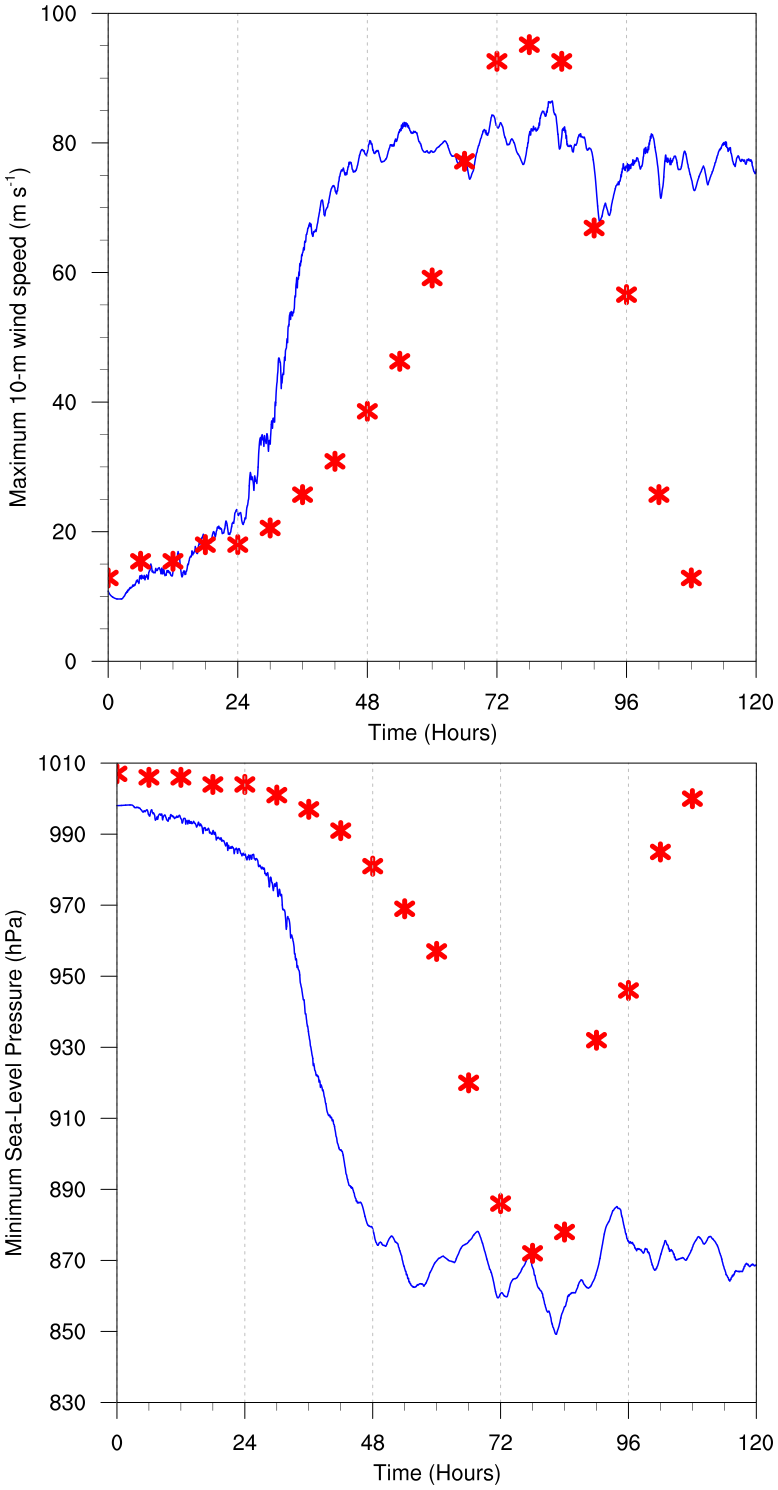
\includegraphics[width=19pc]{figures/vmax+pmin.png}}
\caption{The maximum 10-m wind speed (top panel; m s\textsuperscript{-1}) and minimum sea-level pressure (bottom panel; hPa) in the simulated storm (blue lines) and from Hurricane Patricia's best track (red stars).}
\label{fig:vmax+pmin}
\end{figure}

%FIGURE 2%
\begin{figure}[ht]
\centerline{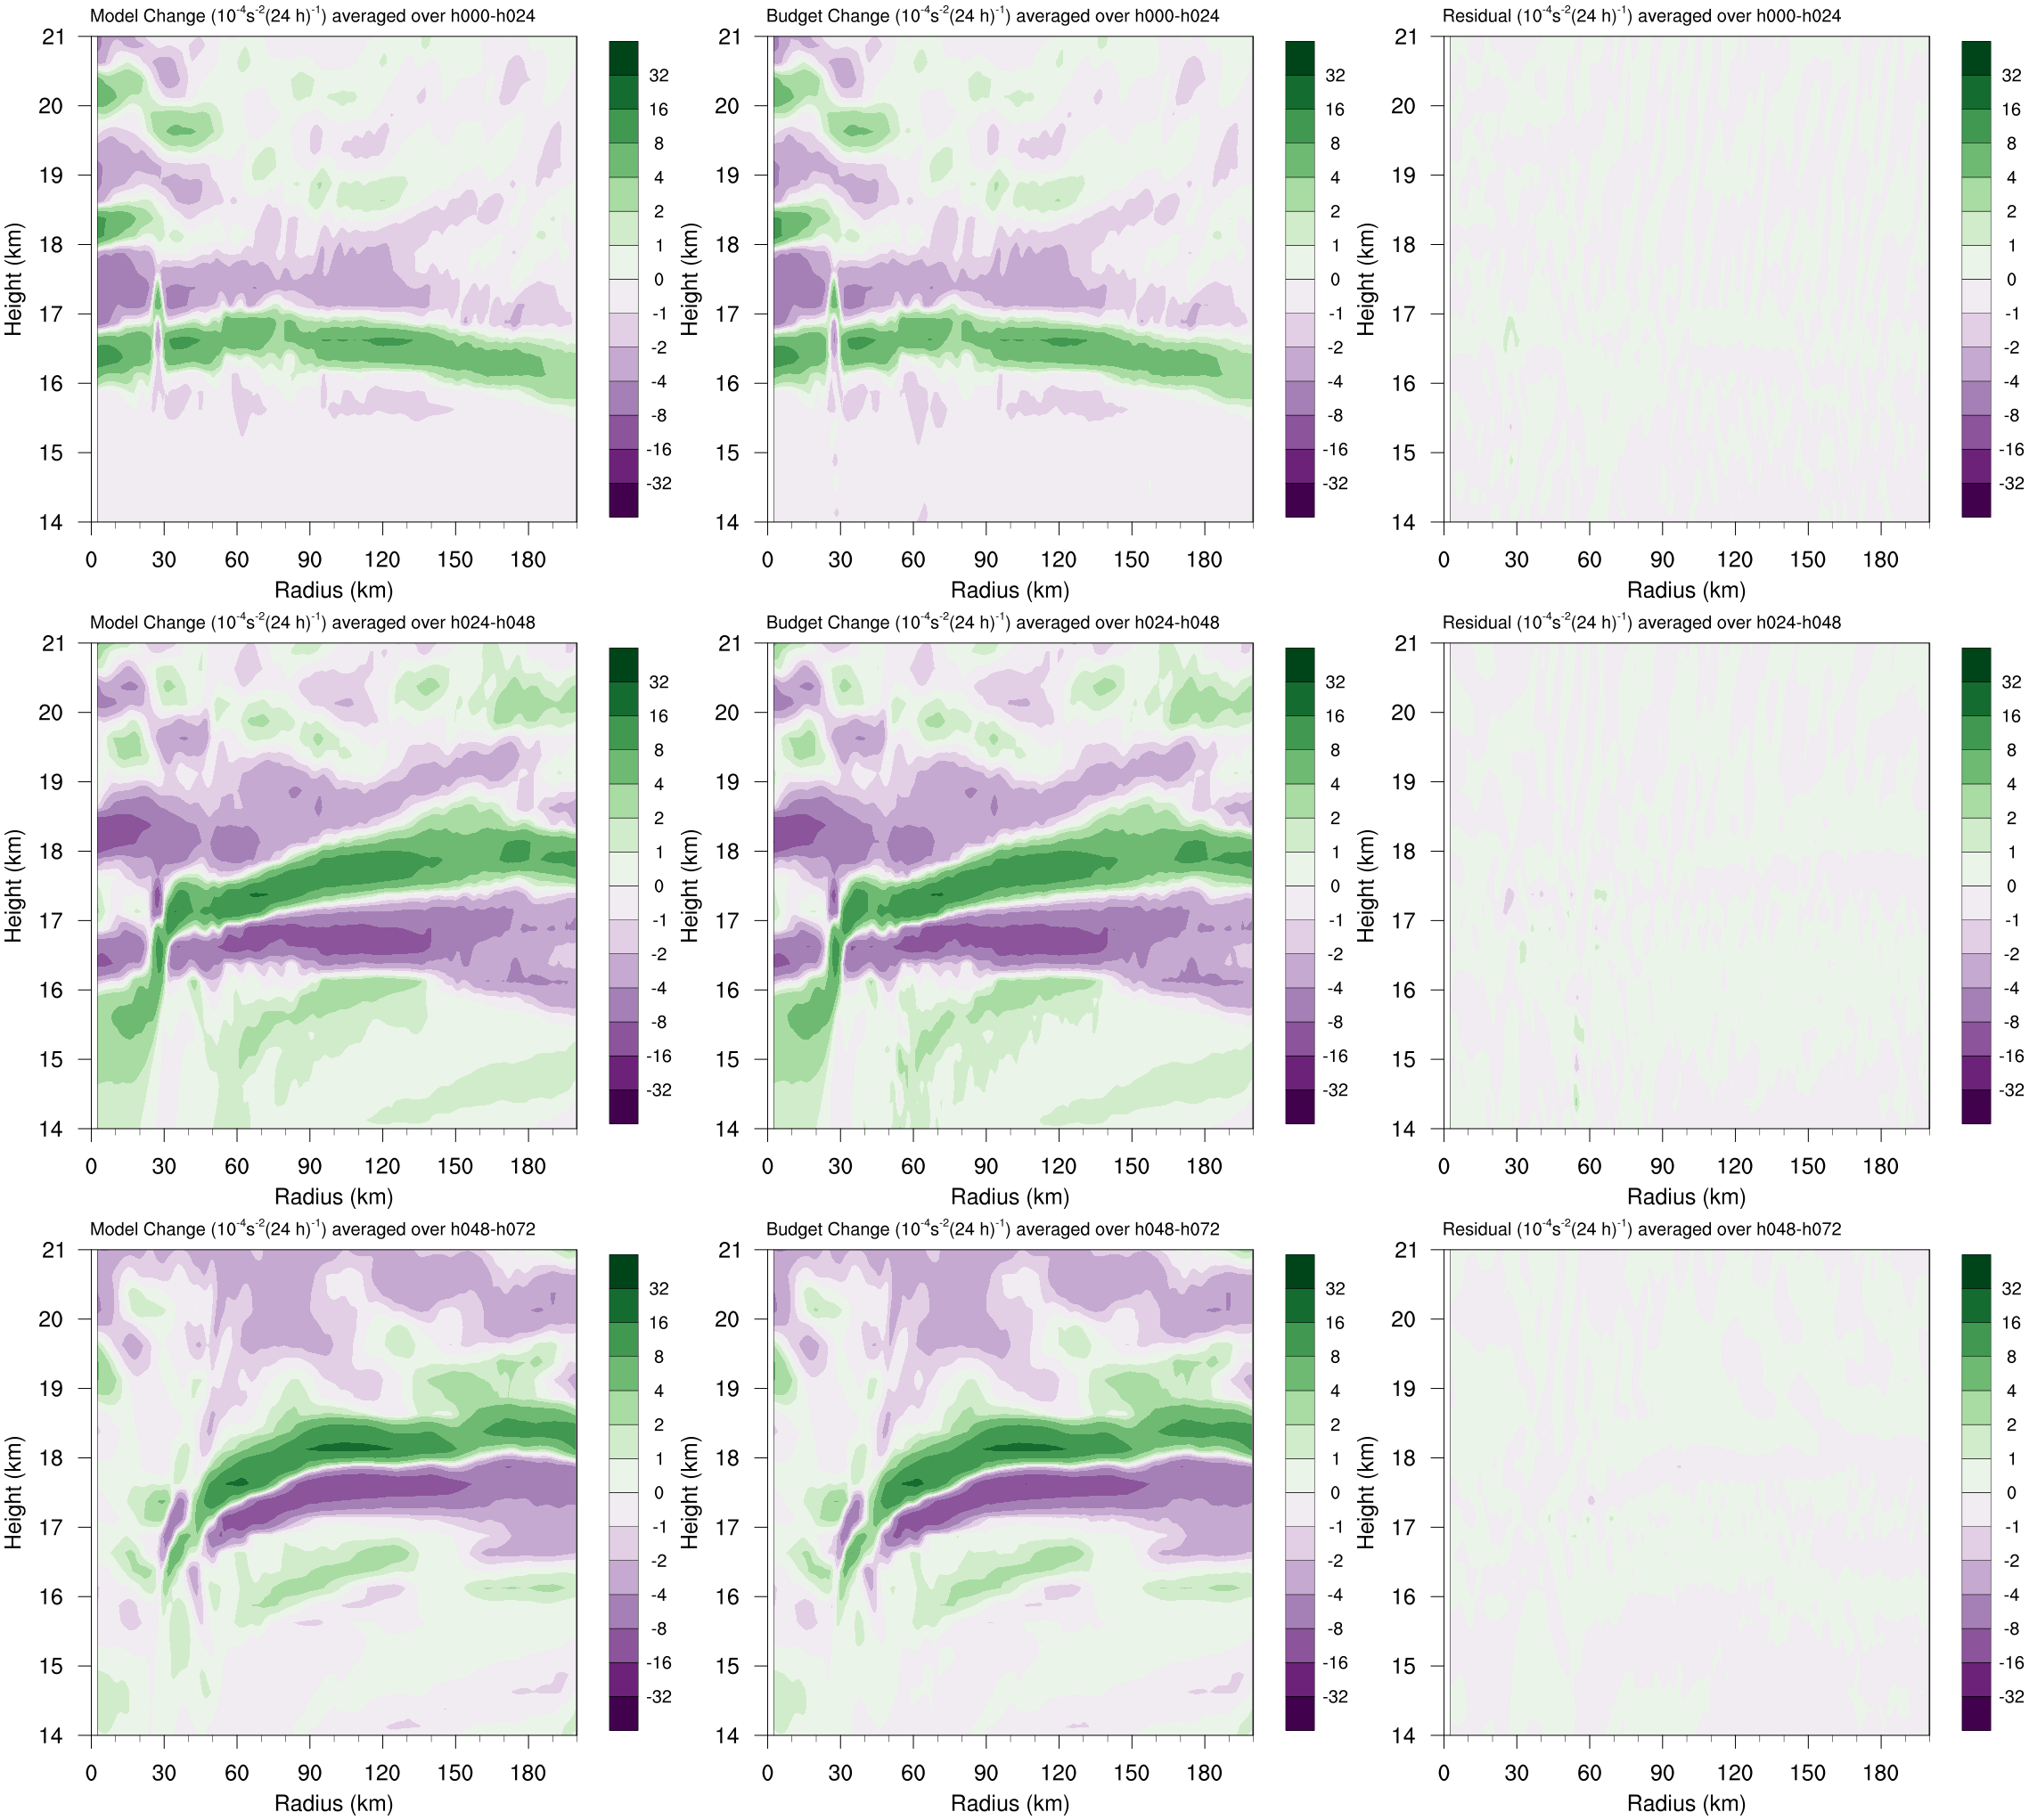
\includegraphics[width=39pc]{figures/mod+bud+res.png}}
\caption{Left panels: Twenty-four-hour changes in squared Brunt-V{\"a}is{\"a}l{\"a} frequency ($N^2$; 10\textsuperscript{-4} s\textsuperscript{-2}) over (top row) 0-24 hours, (middle row) 24-48 hours, (bottom row) 48-72 hours.
Middle Panels: The $N^2$ change over the same time periods computed using Eqs. \ref{eq:dn2dt}-\ref{eq:budgetchange}, %together with Eqs. \ref{eq:dn2dt}, \ref{eq:dthetadt}.
Right Panels: The budget residual over the same time periods, computed by subtracting the budget change (middle column) from the model change (left column).}
\label{fig:mod+bud+res}
\end{figure}

%FIGURE 3%
\begin{figure*}[ht]
\centerline{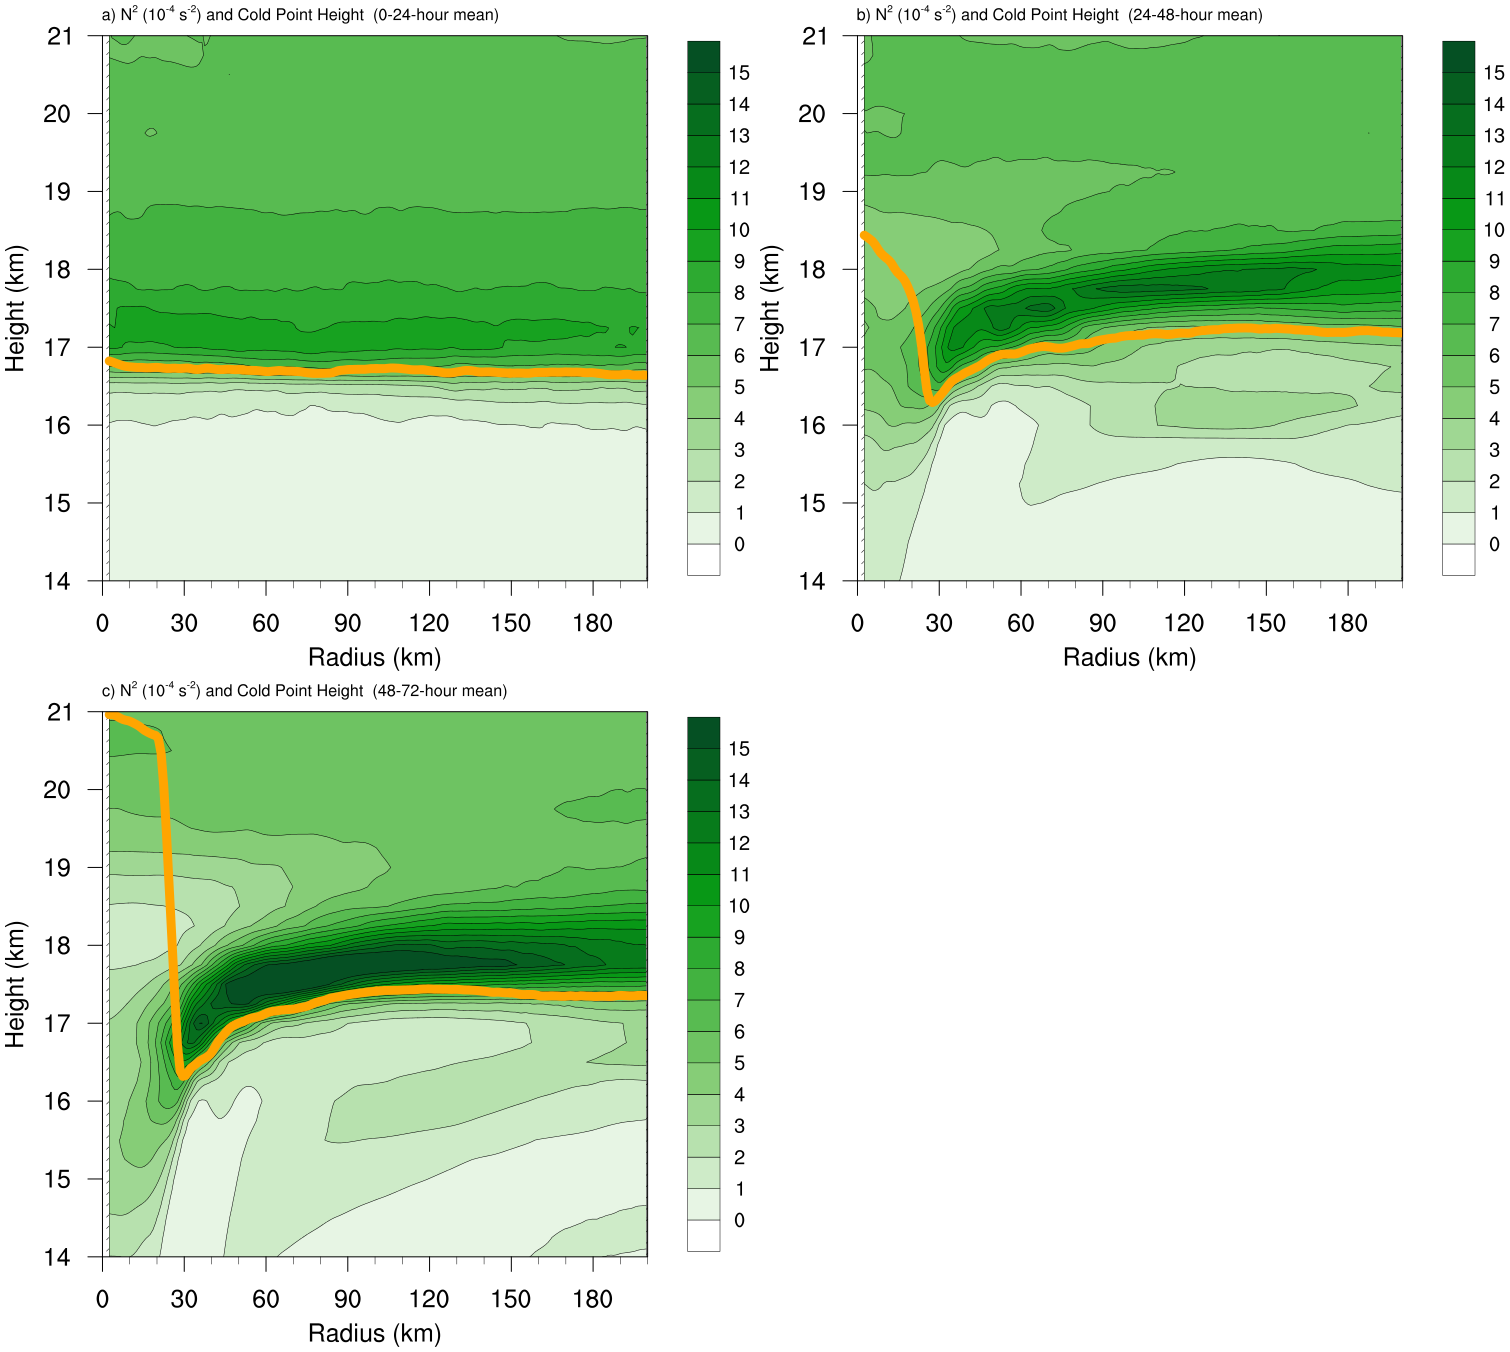
\includegraphics[width=39pc]{figures/n2-24hr-avgs.png}}
\caption{Twenty-four-hour averages of squared Brunt-V{\"a}is{\"a}l{\"a} frequency ($N^2$; 10\textsuperscript{-4} s\textsuperscript{-2}) over (a) 0-24 hours, (b) 24-48 hours, (c) 48-72 hours.
Orange lines represent the cold-point tropopause averaged over the same time periods.}
\label{fig:n2-24hr-avgs}
\end{figure*}

%FIGURE 4%
\begin{figure}[ht]
\centerline{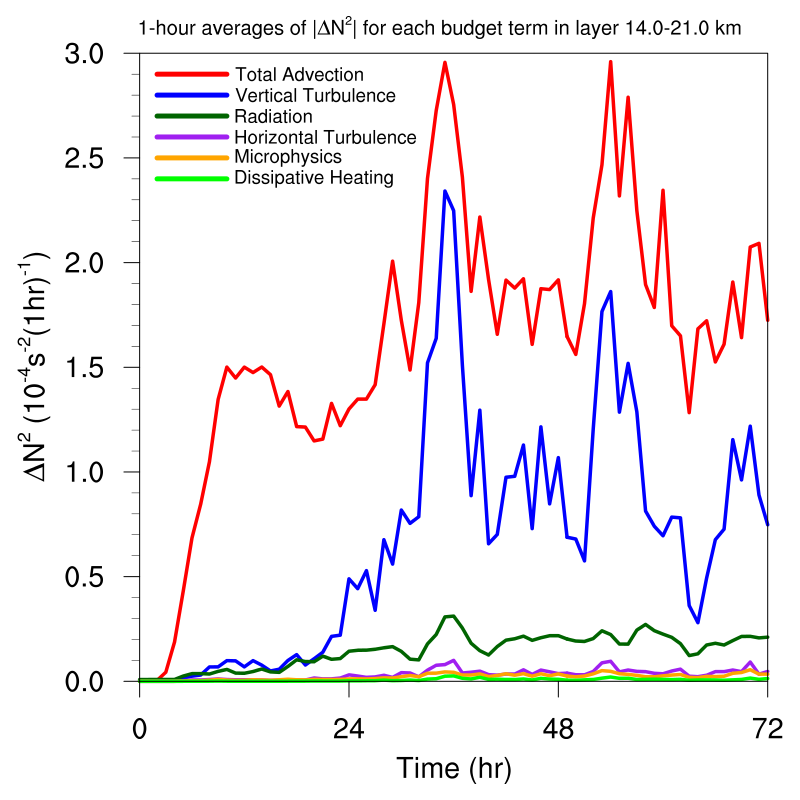
\includegraphics[width=19pc]{figures/AVG_budterms.png}}
\caption{Time series of the contribution of each of the budget terms to the time tendency of the squared Brunt-V{\"a}is{\"a}l{\"a} frequency ($N^2$; 10\textsuperscript{-4} s\textsuperscript{-2}).
For each budget term, the absolute value of the $N^2$ tendency is averaged temporally over 1-hour periods (using output every minute), and spatially in a region extending from 0 to 200 km radius and 14 to 21 km altitude.}
\label{fig:avgbudterms}
\end{figure}

%FIGURE 5%
\begin{figure*}[ht]
\centerline{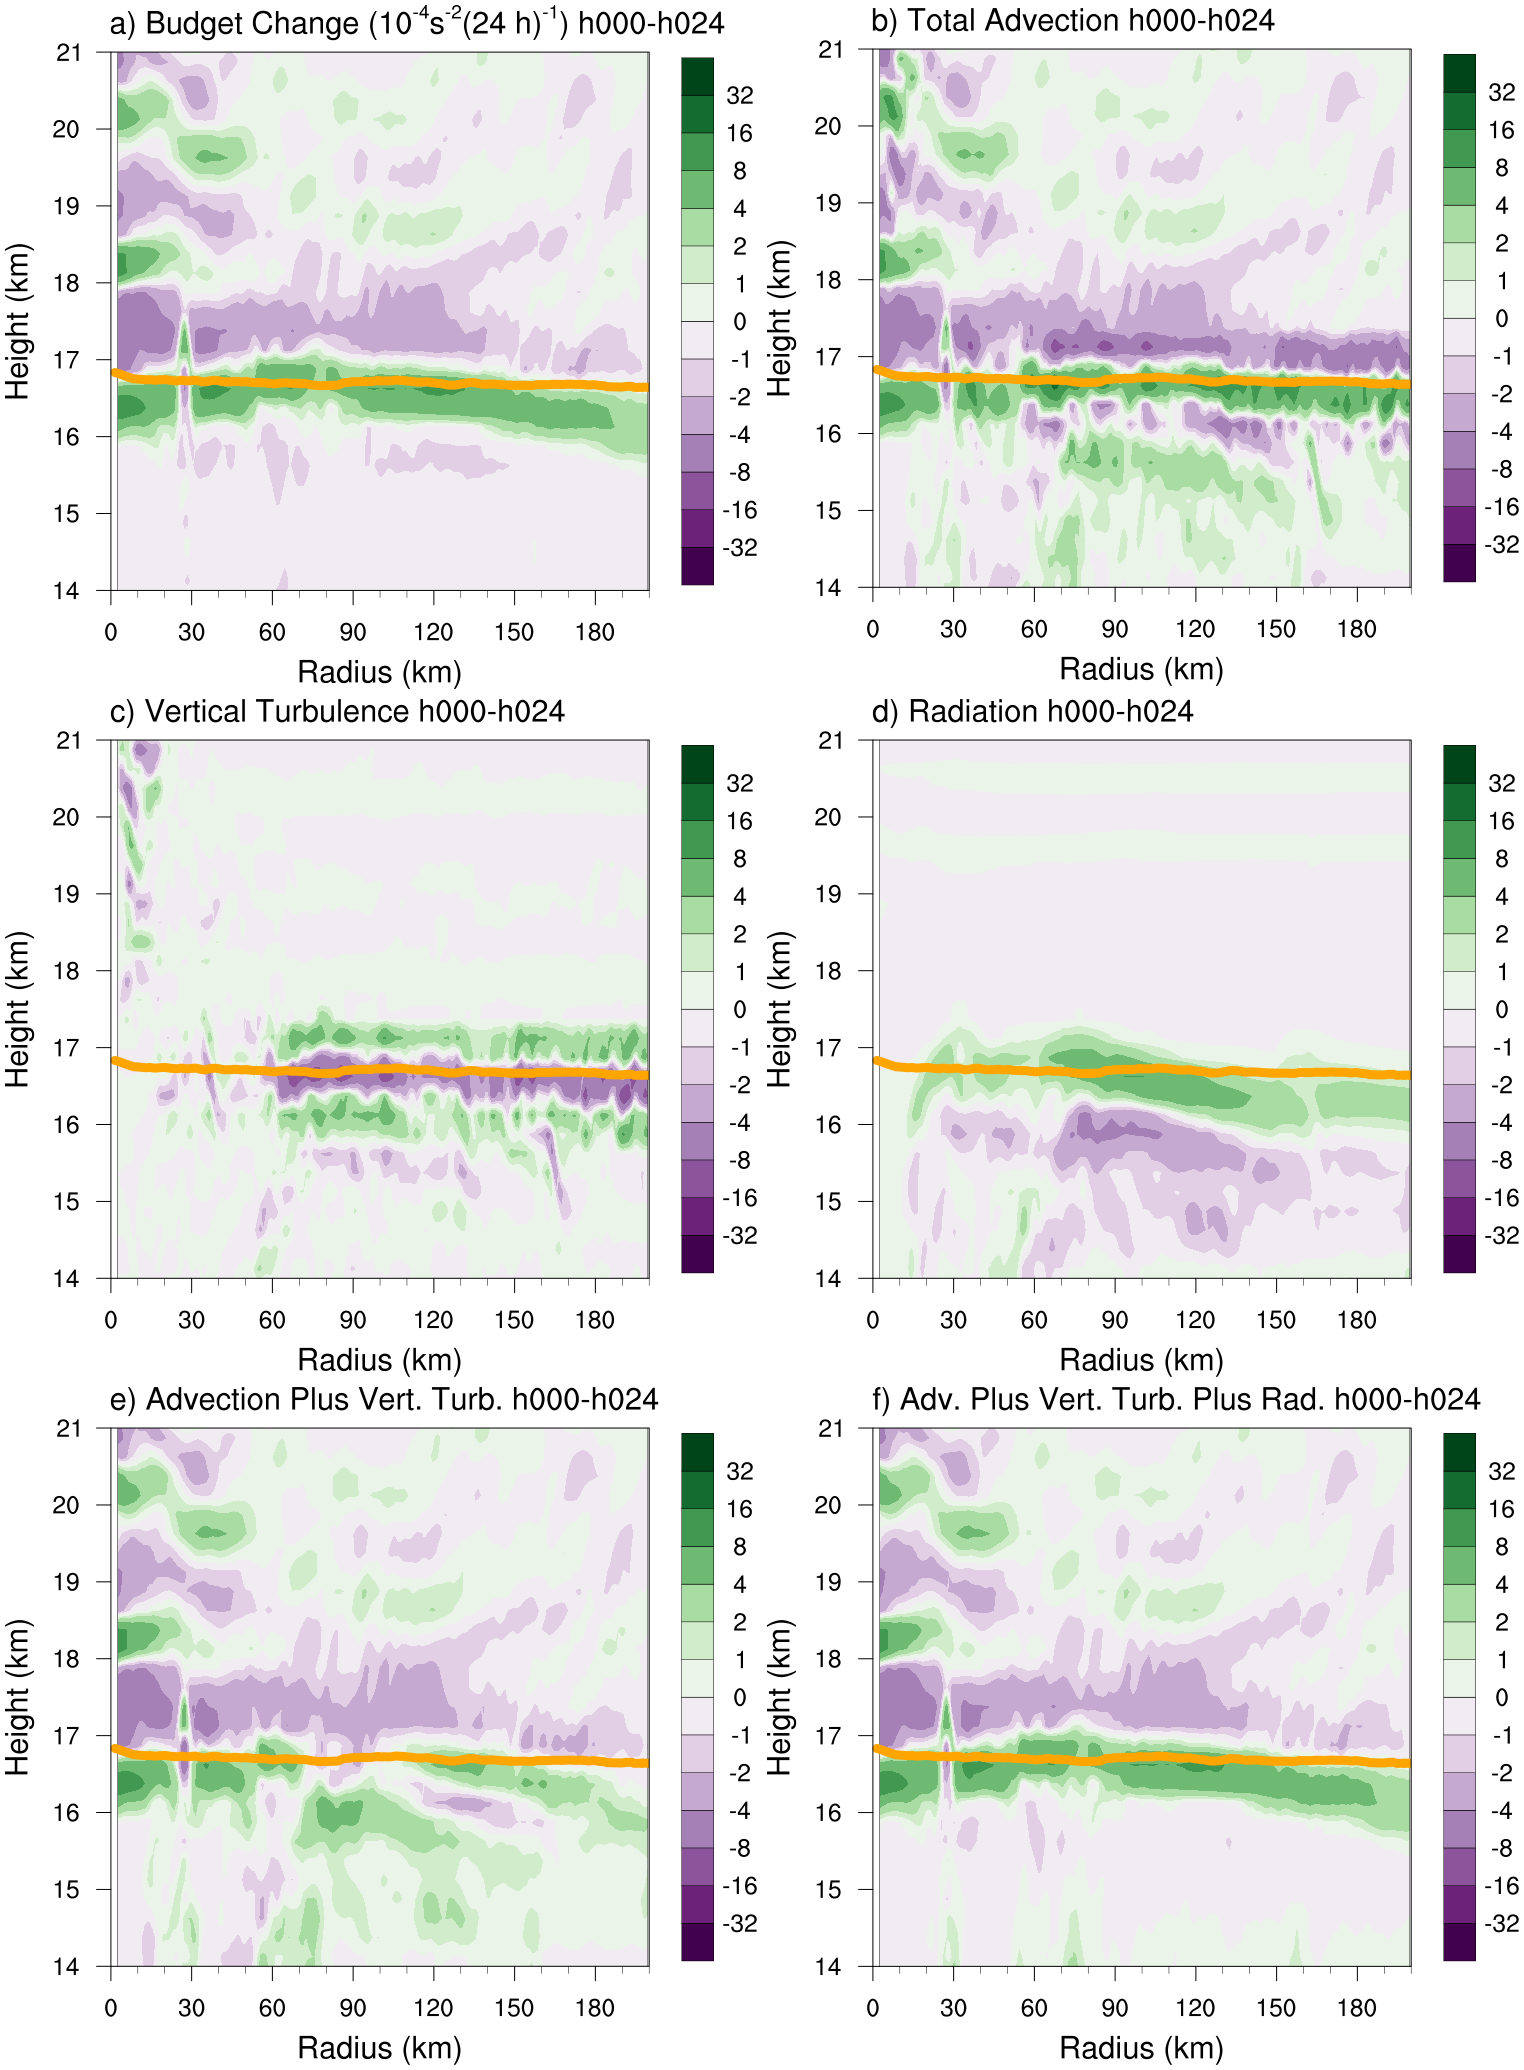
\includegraphics[width=39pc]{figures/h000-h024-budgetterms.png}}
\end{figure*}
\begin{figure}
\caption{(a) Total change in $N^2$ over the 0-24-hour period (10\textsuperscript{-4} s\textsuperscript{-2} (24 h)\textsuperscript{-1}) and the contributions to that change from (b) the sum of horizontal and vertical advection, (c) vertical turbulence, (d) longwave and shortwave radiation, (e) the sum of horizontal advection, vertical advection, and vertical turublence, and (f) the sum of horizontal advection, vertical advection, vertical turbulence, and longwave and shortwave radiation.}
\label{fig:stab-00-24}
\end{figure}

%FIGURE 6%
\begin{figure*}[ht]
\centerline{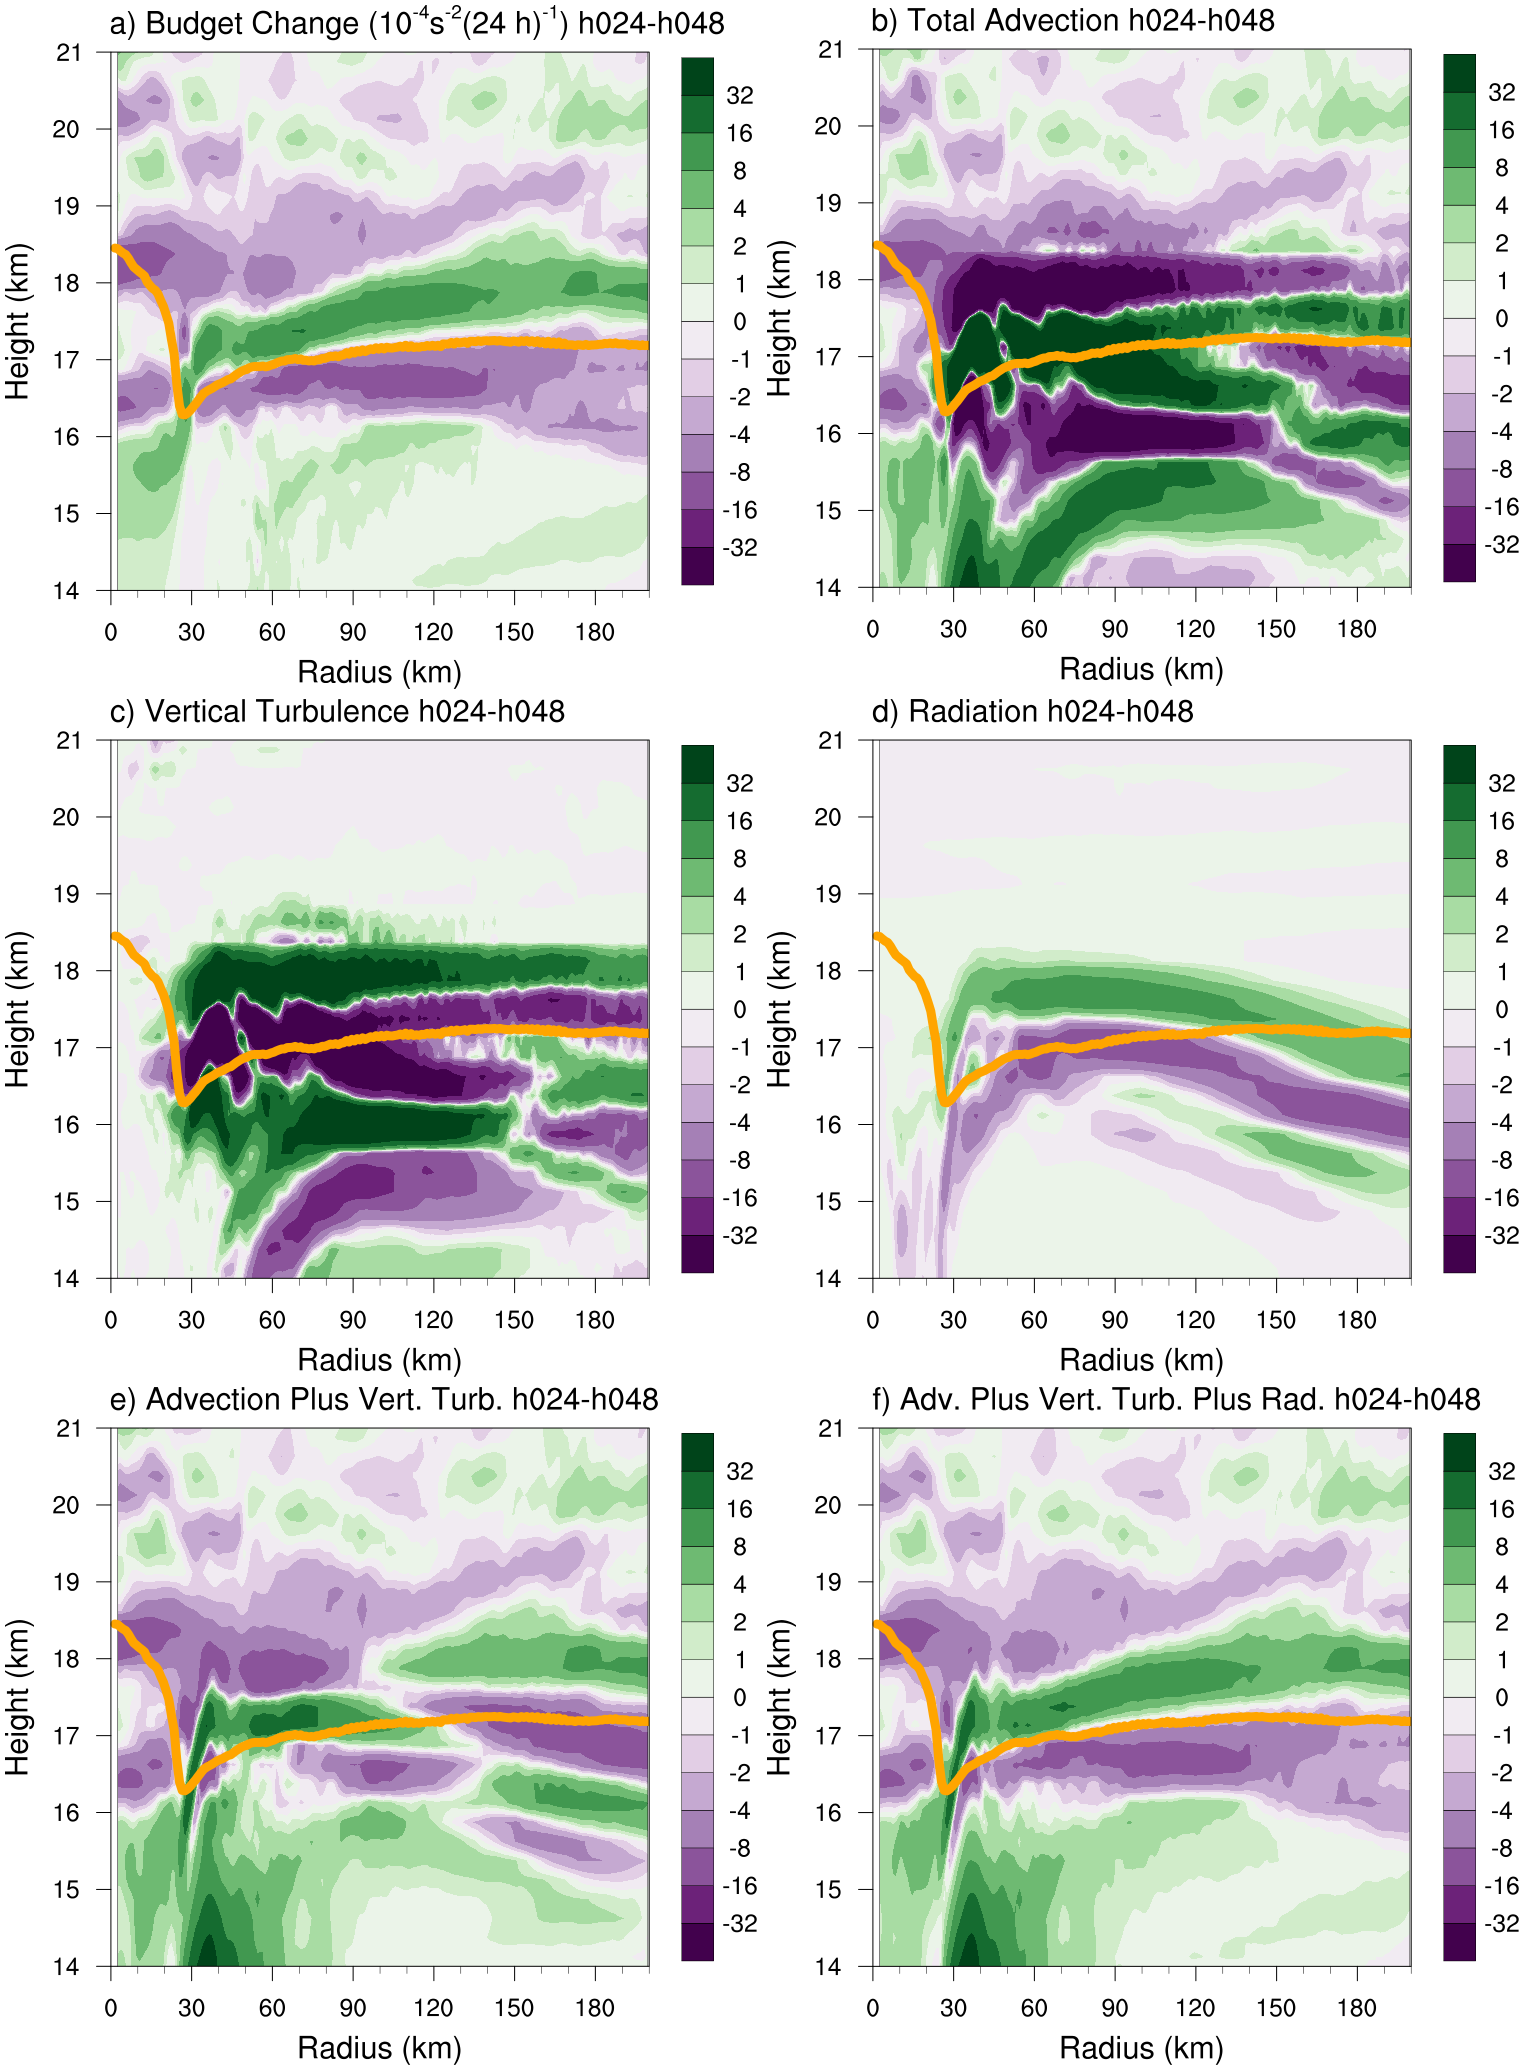
\includegraphics[width=39pc]{figures/h024-h048-budgetterms.png}}
\caption{As in Fig.~\ref{fig:stab-00-24}, but for the 24-48-hour period.}
\label{fig:stab-24-48}
\end{figure*}

%FIGURE 7%
\begin{figure*}[ht]
\centerline{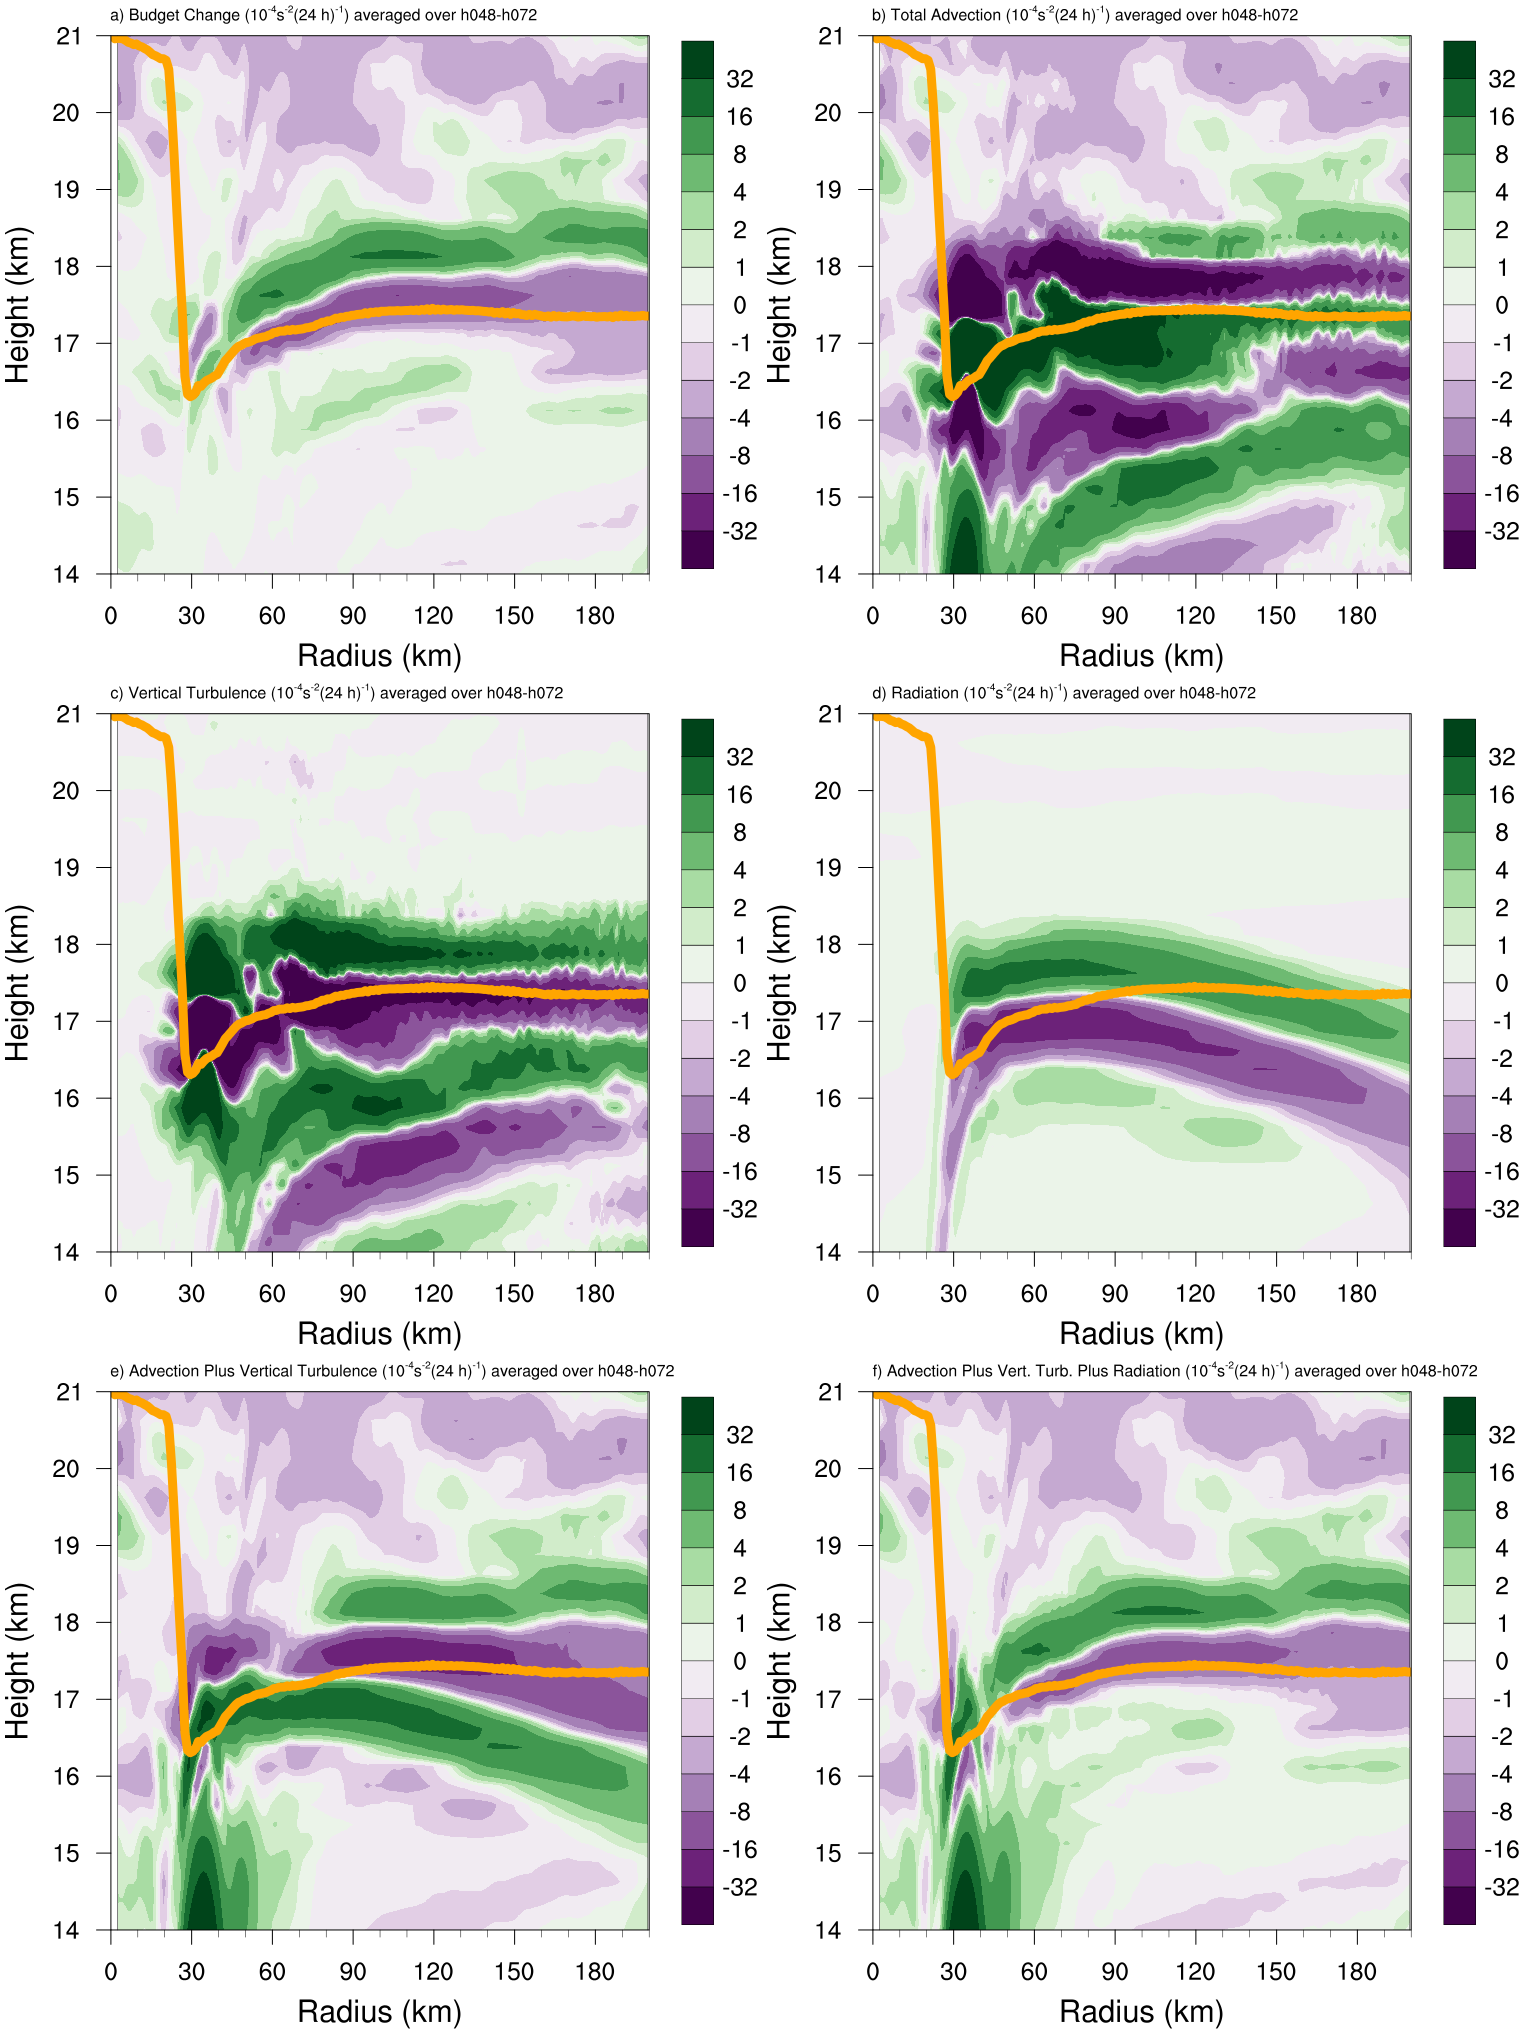
\includegraphics[width=39pc]{figures/h048-h072-budgetterms.png}}
\caption{As in Fig.~\ref{fig:stab-00-24}, but for the 48-72-hour period.}
\label{fig:stab-48-72}
\end{figure*}

%FIGURE 8%
%\begin{figure*}[ht]
%\centerline{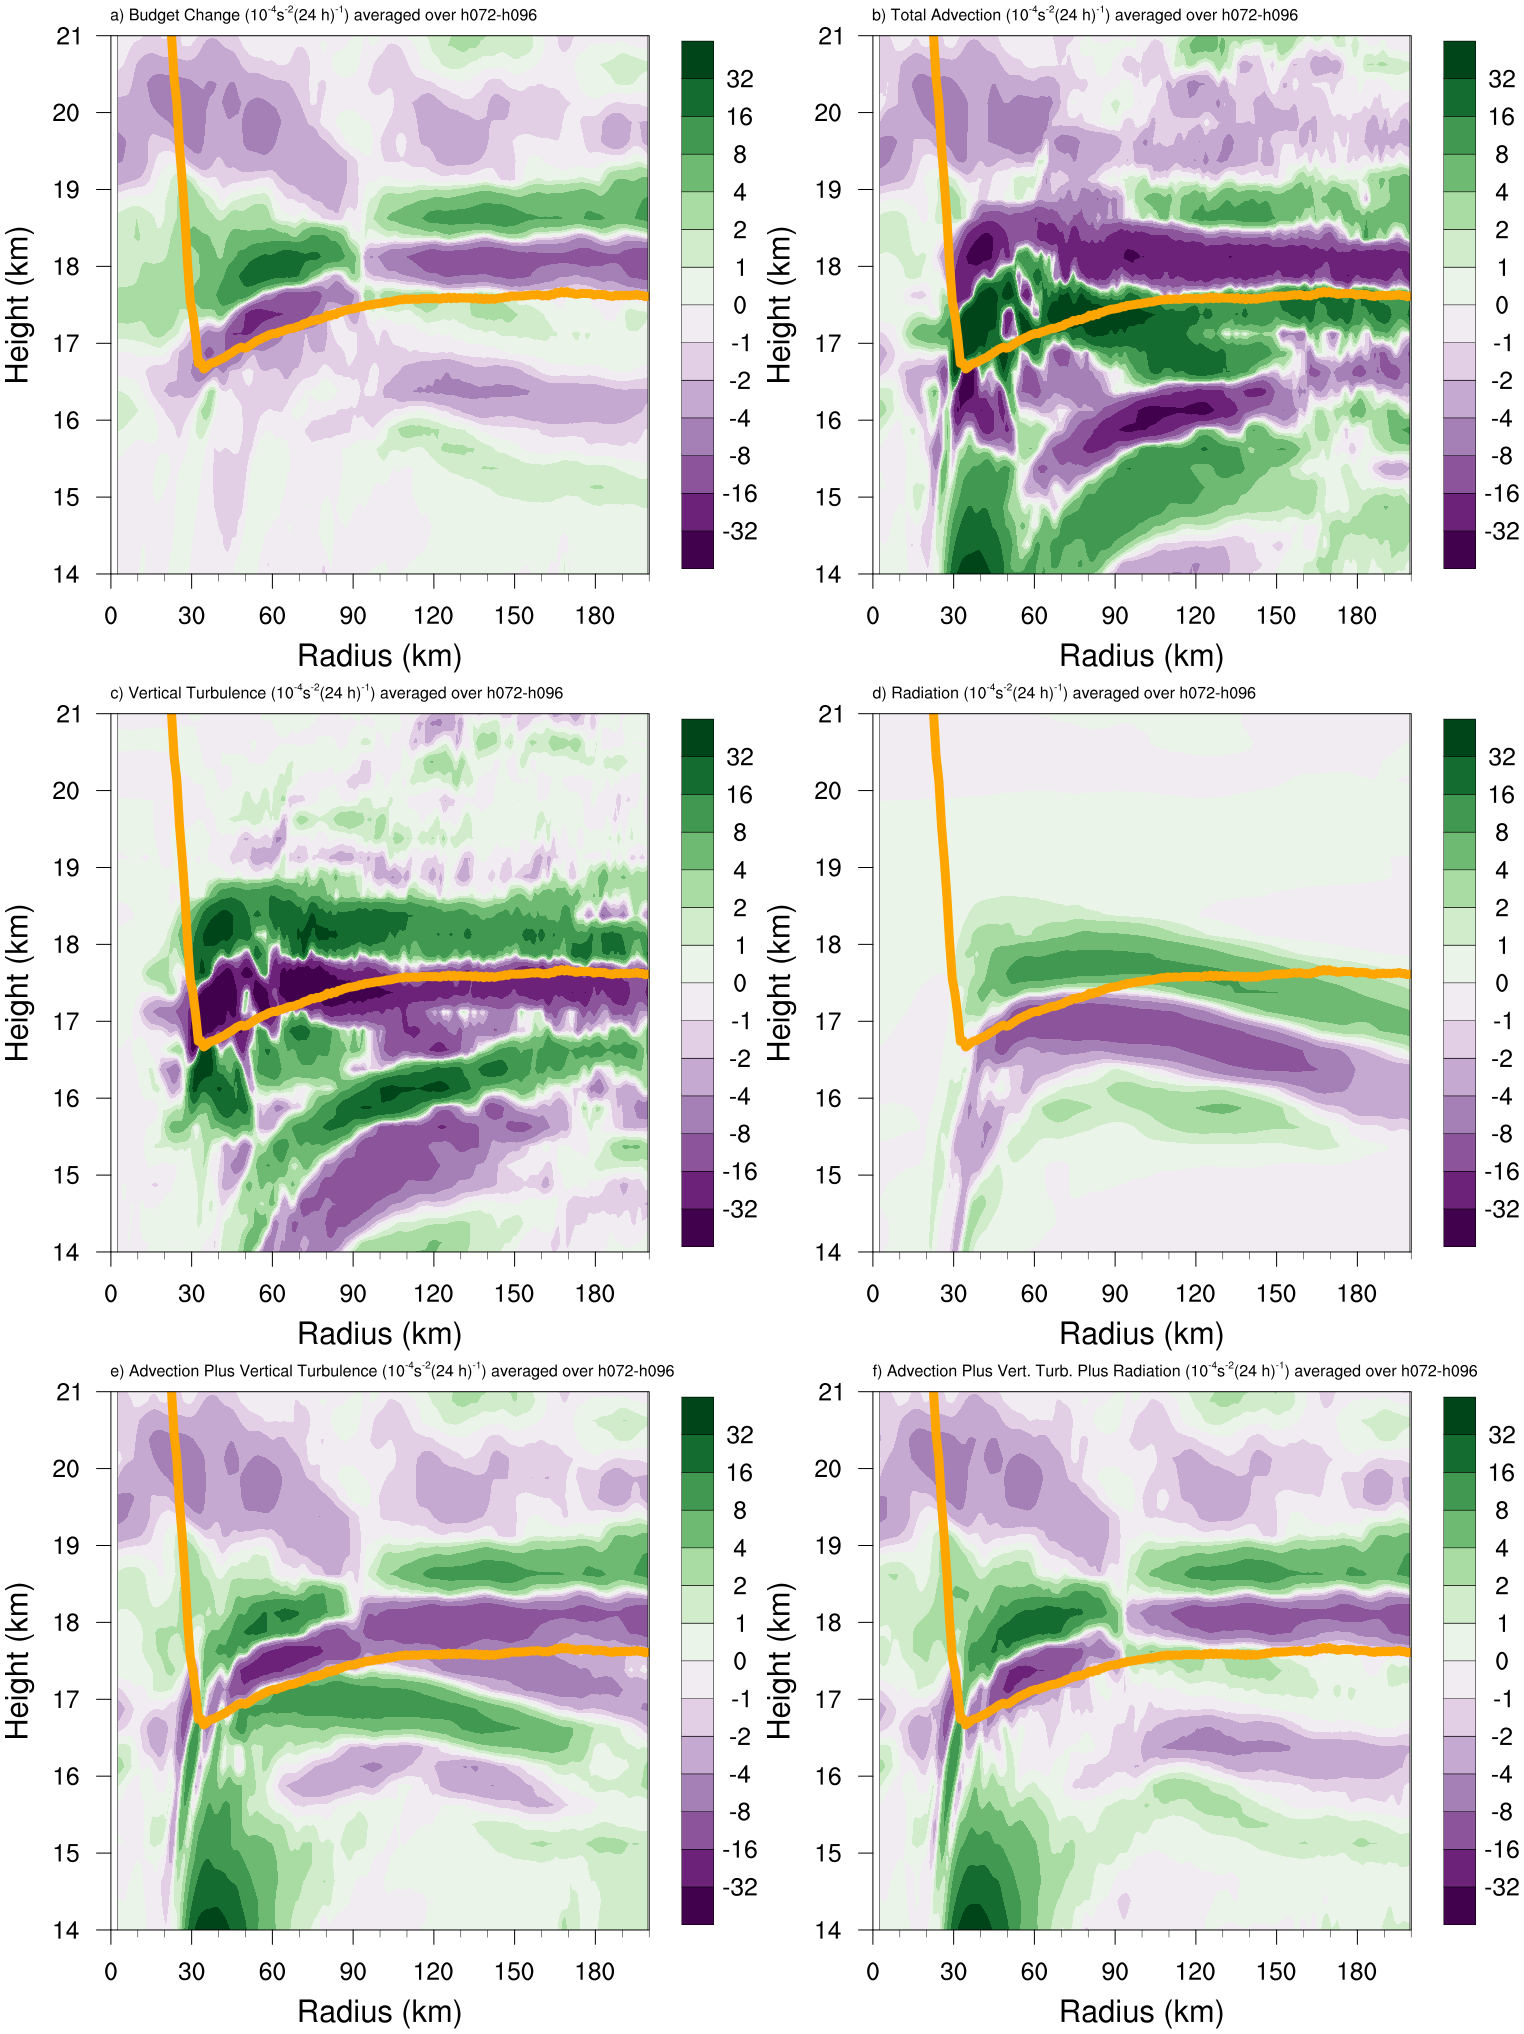
\includegraphics[width=33pc]{figures/h072-h096-budgetterms.png}}
%\caption{As in Fig.~\ref{fig:stab-48-72}, but for the 72-96-hour period.}
%\label{fig:stab-72-96}
%\end{figure*}

%FIGURE 8%
%\begin{figure*}[ht]
%\centerline{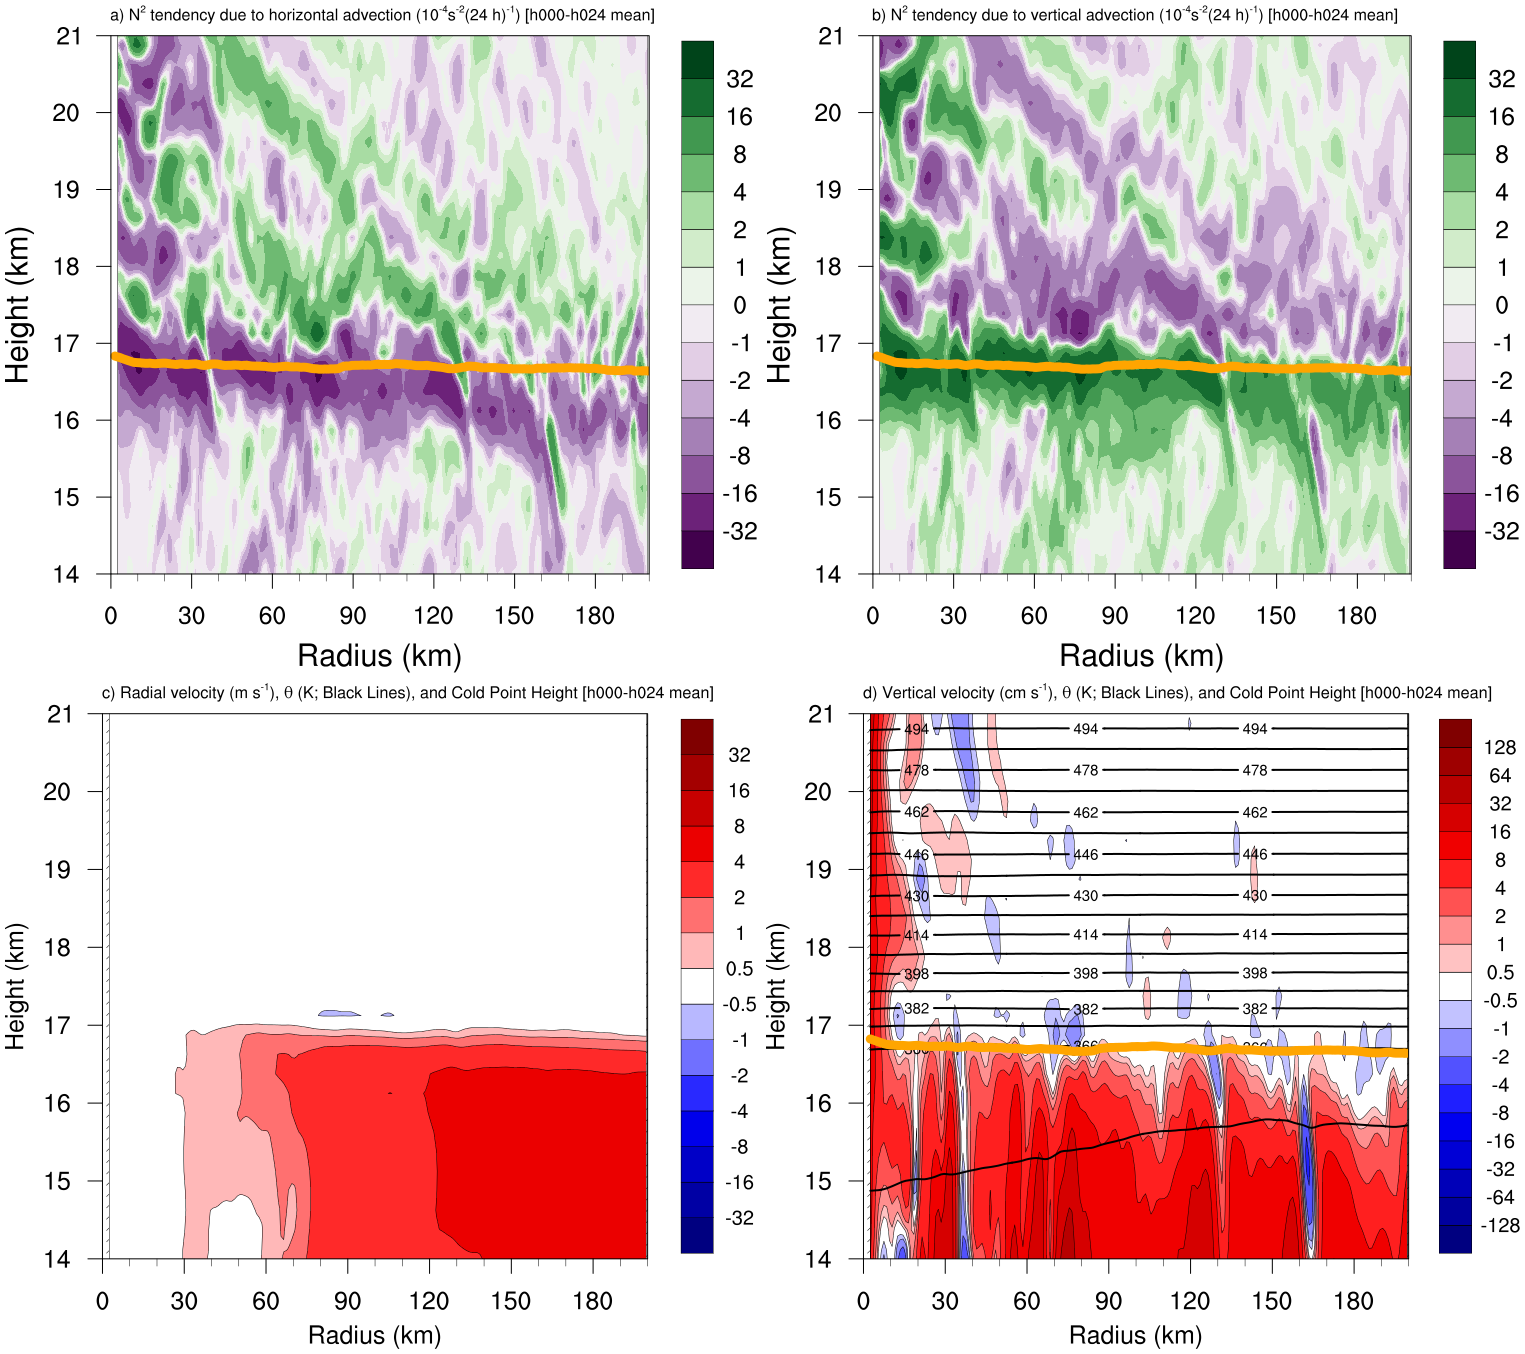
\includegraphics[width=39pc]{figures/h000-h024-adv.png}}
%\caption{The contribution to the change in $N^2$ over the 0-24-hour period (10\textsuperscript{-4} s\textsuperscript{-2} (24 hr)\textsuperscript{-1}) by (a) horizontal advection and (b) vertical advection. (c) The radial velocity (m s\textsuperscript{-1}; filled contours), potential temperature (K; thick black contours), and cold-point tropopause height (orange line) averaged over the 0-24-hour period. (d) The vertical velocity (cm s\textsuperscript{-1}; filled contours), potential temperature (K; thick black contours), and cold-point tropopause height (orange line) averaged over the 0-24-hour period.}
%\label{fig:adv-00-24}
%\end{figure*}


%FIGURE 8%
%\begin{figure*}[ht]
%\centerline{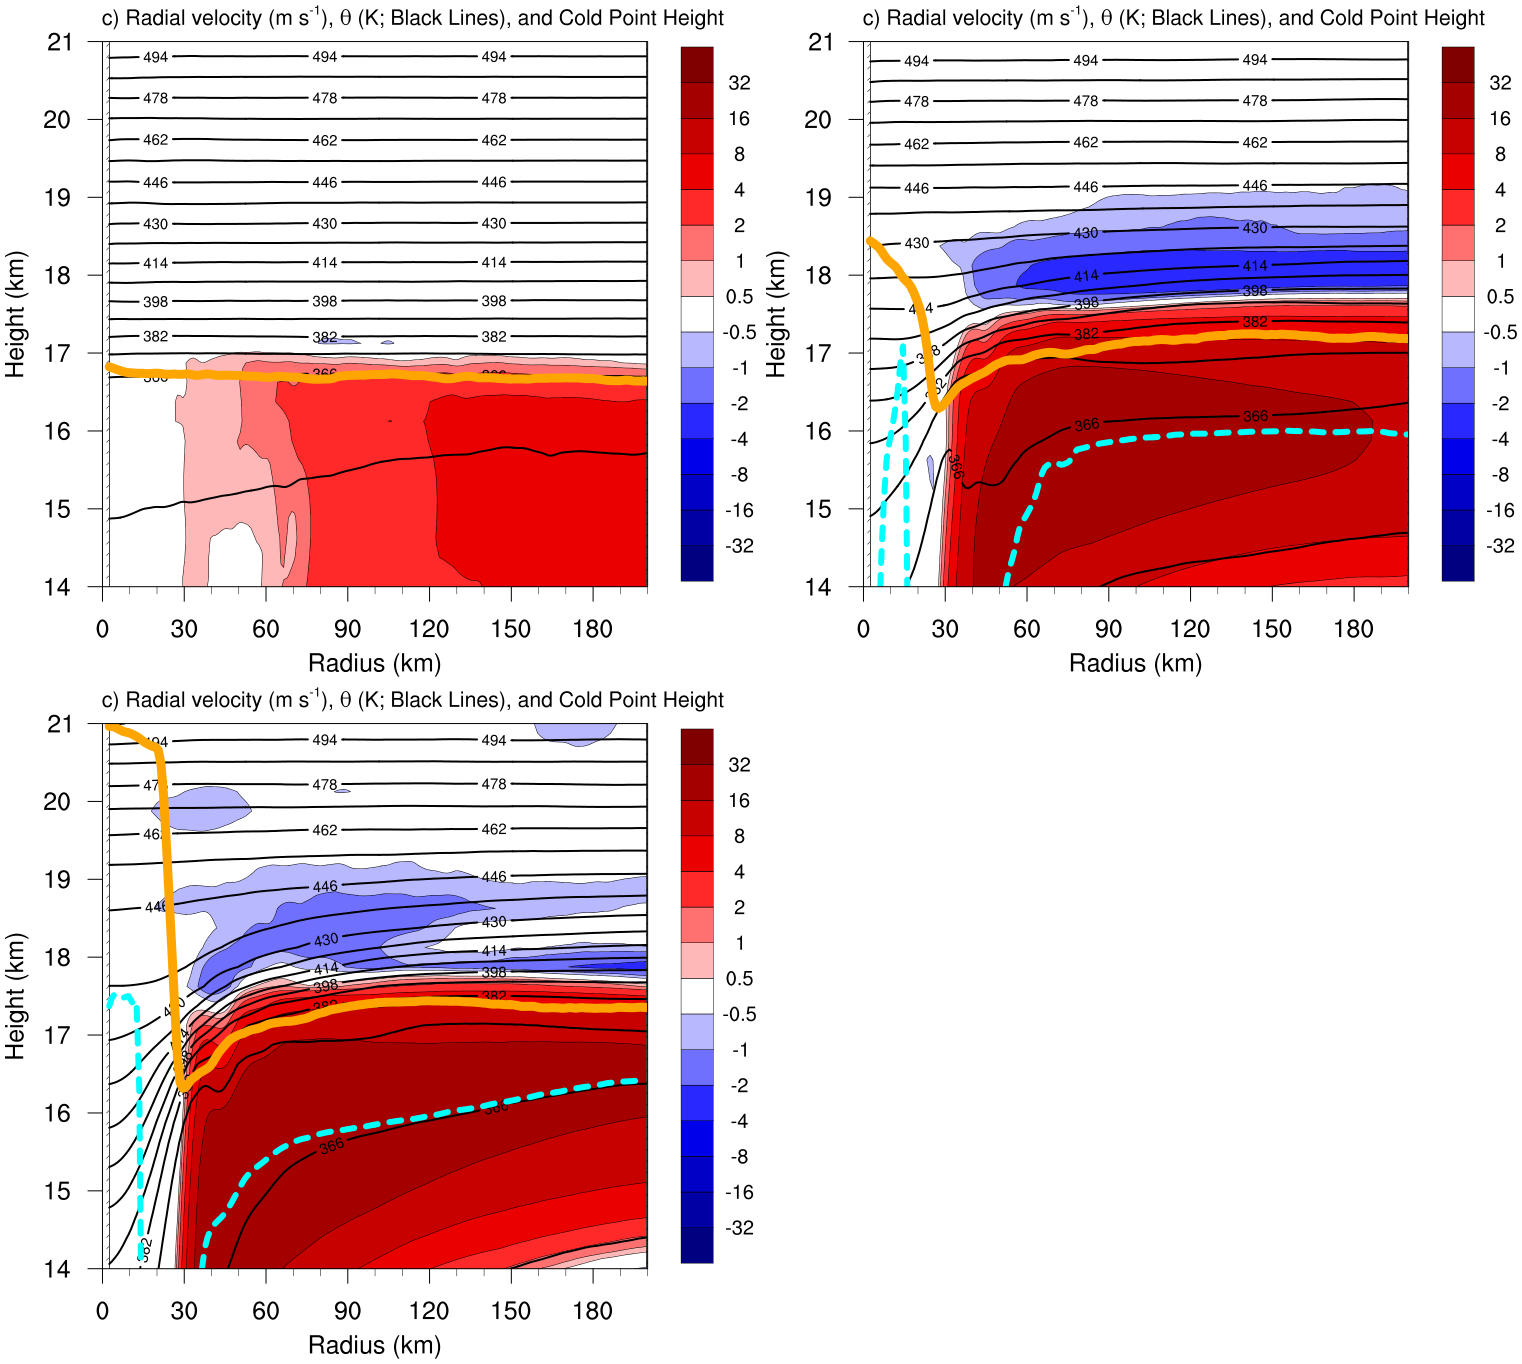
\includegraphics[width=39pc]{figures/u.png}}
%\caption{Radial velocity (m s\textsuperscript{-1}; filled contours), potential temperature (K; thick black contours), and cold-point tropopause height (orange lines) averaged over (a) 0-24 hours, (b) 24-48 hours, and (c) 48-72 hours.}
%\label{fig:u}
%\end{figure*}

%FIGURE 8%
\begin{figure*}[ht]
\centerline{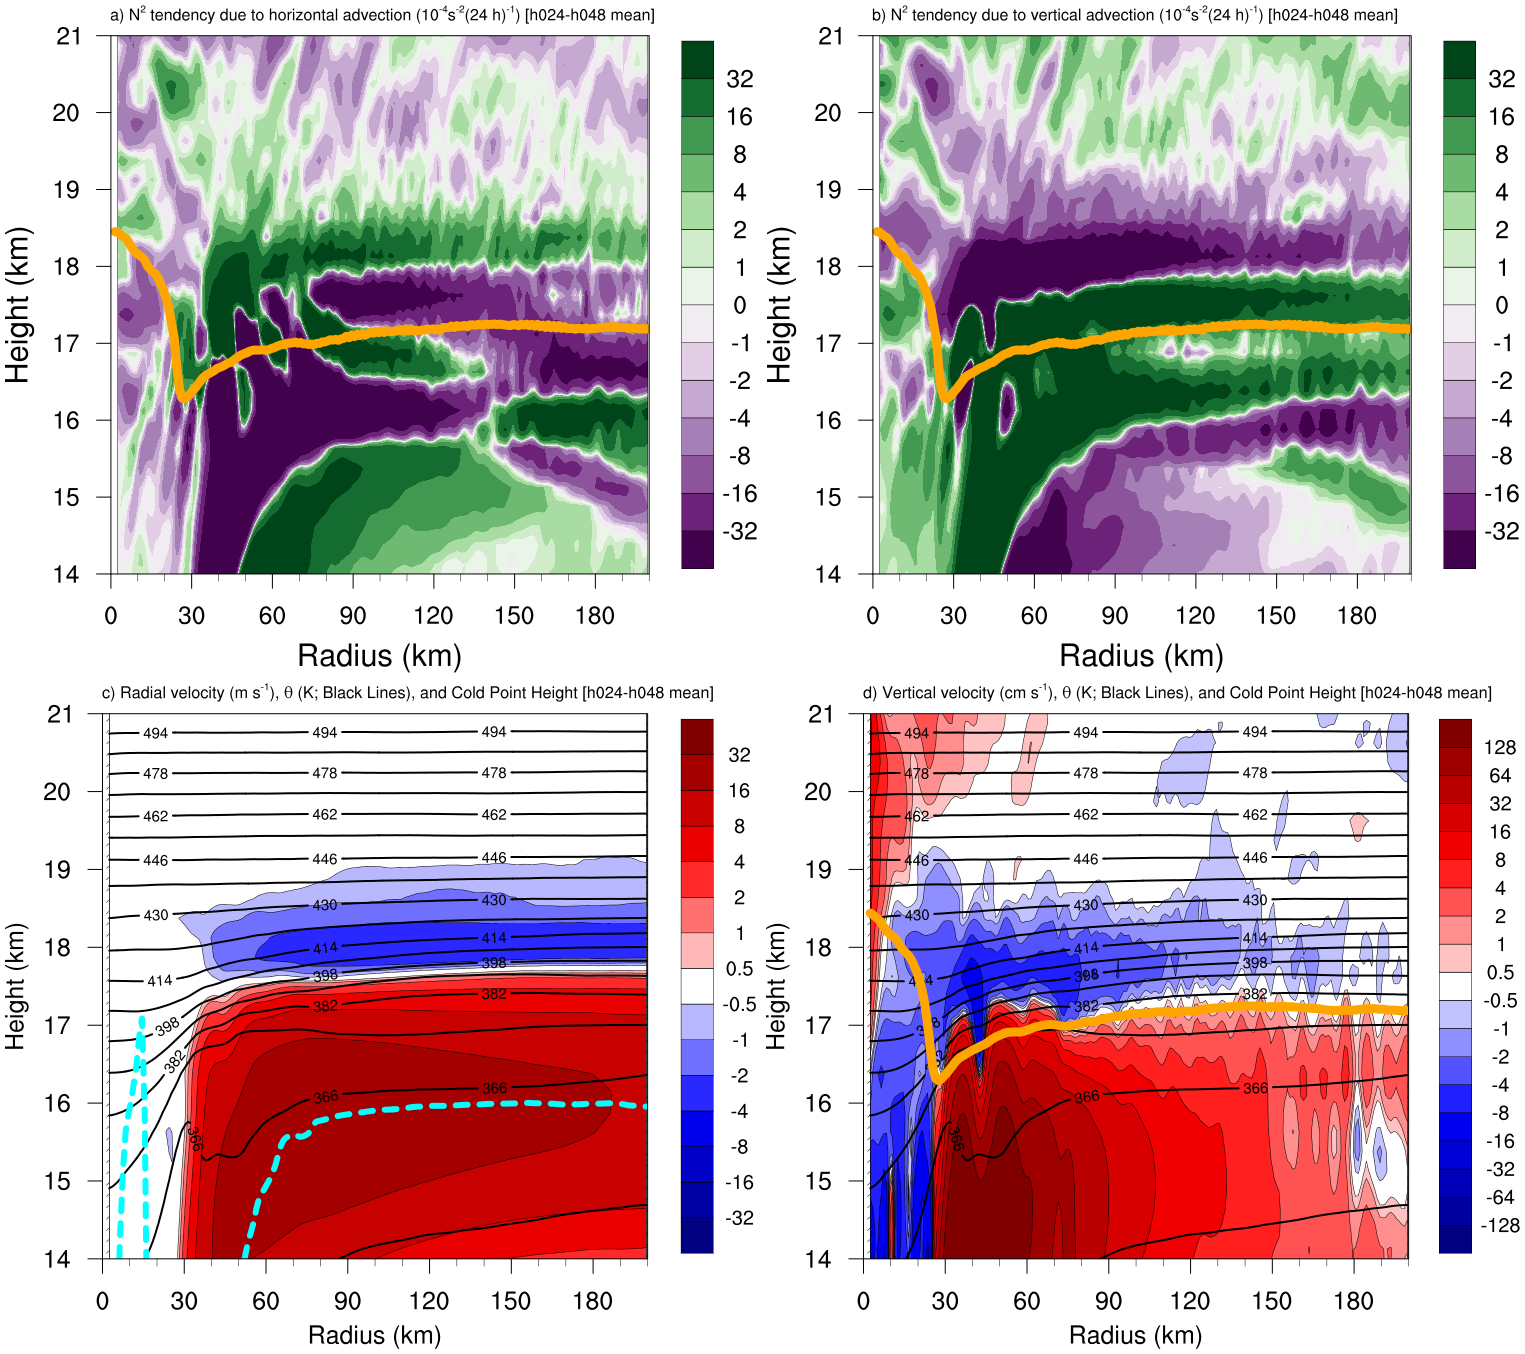
\includegraphics[width=39pc]{figures/h024-h048-adv.png}}
\caption{The contribution to the change in $N^2$ over the 24-48-hour period (10\textsuperscript{-4} s\textsuperscript{-2} (24 h)\textsuperscript{-1}) by (a) horizontal advection and (b) vertical advection. (c) The radial velocity (m s\textsuperscript{-1}; filled contours), potential temperature (K; thick black contours), cold-point tropopause height (orange line), and level of maximum outflow (dashed cyan line) averaged over the 24-48-hour period. (d) The vertical velocity (cm s\textsuperscript{-1}; filled contours), potential temperature (K; thick black contours), and cold-point tropopause height (orange line) averaged over the 24-48-hour period.}
%\caption{As in Fig. \ref{fig:adv-00-24}, but for the 24-48-hour period.}
\label{fig:adv-24-48}
\end{figure*}

%FIGURE 9%
%\begin{figure*}[ht]
%\centerline{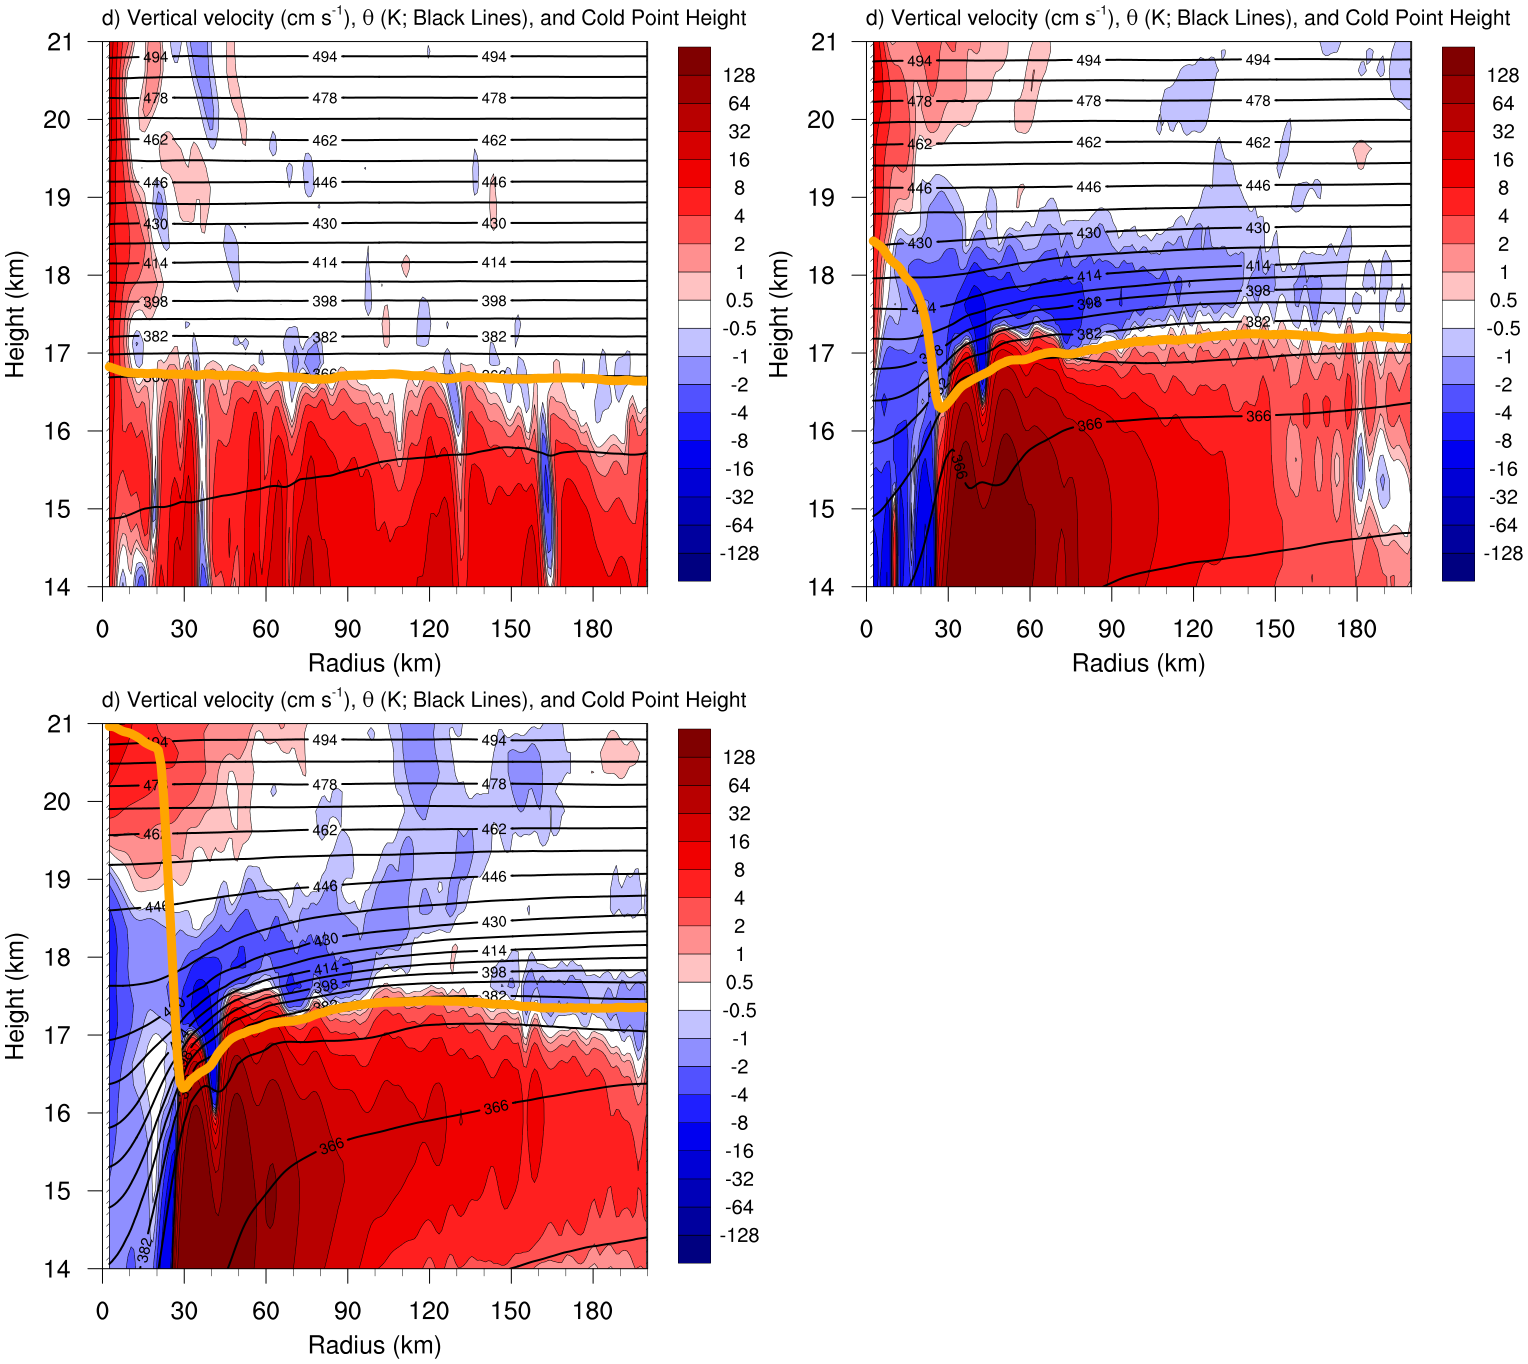
\includegraphics[width=39pc]{figures/w.png}}
%\caption{Vertical velocity (cm s\textsuperscript{-1}; filled contours), potential temperature (K; thick black contours), and cold-point tropopause height (orange lines) averaged over (a) 0-24 hours, (b) 24-48 hours, and (c) 48-72 hours.}
%\label{fig:w}
%\end{figure*}

%FIGURE 10%
%\begin{figure*}[ht]
%\centerline{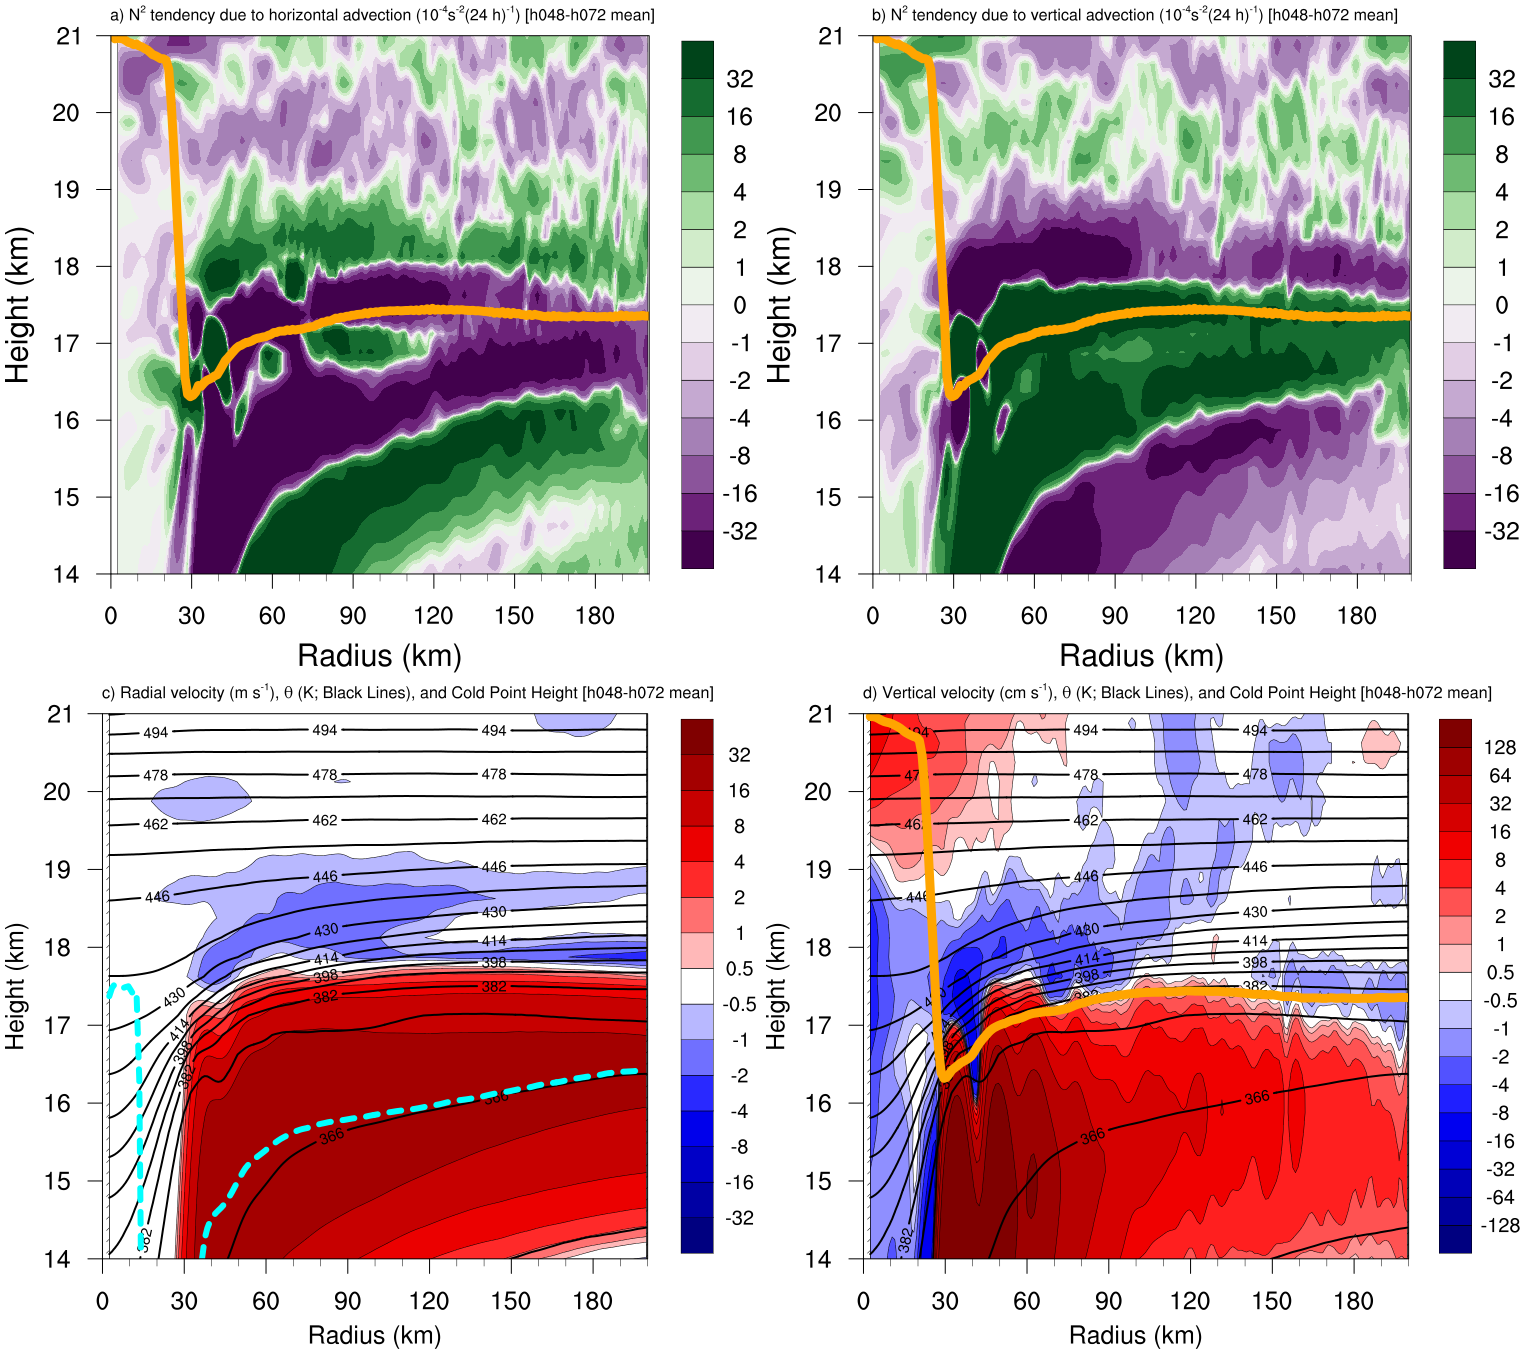
\includegraphics[width=39pc]{figures/h048-h072-adv.png}}
%\caption{As in Fig. \ref{fig:adv-00-24}, but for the 48-72-hour period.}
%\label{fig:adv-48-72}
%\end{figure*}

%FIGURE 9%
\begin{figure*}[ht]
\centerline{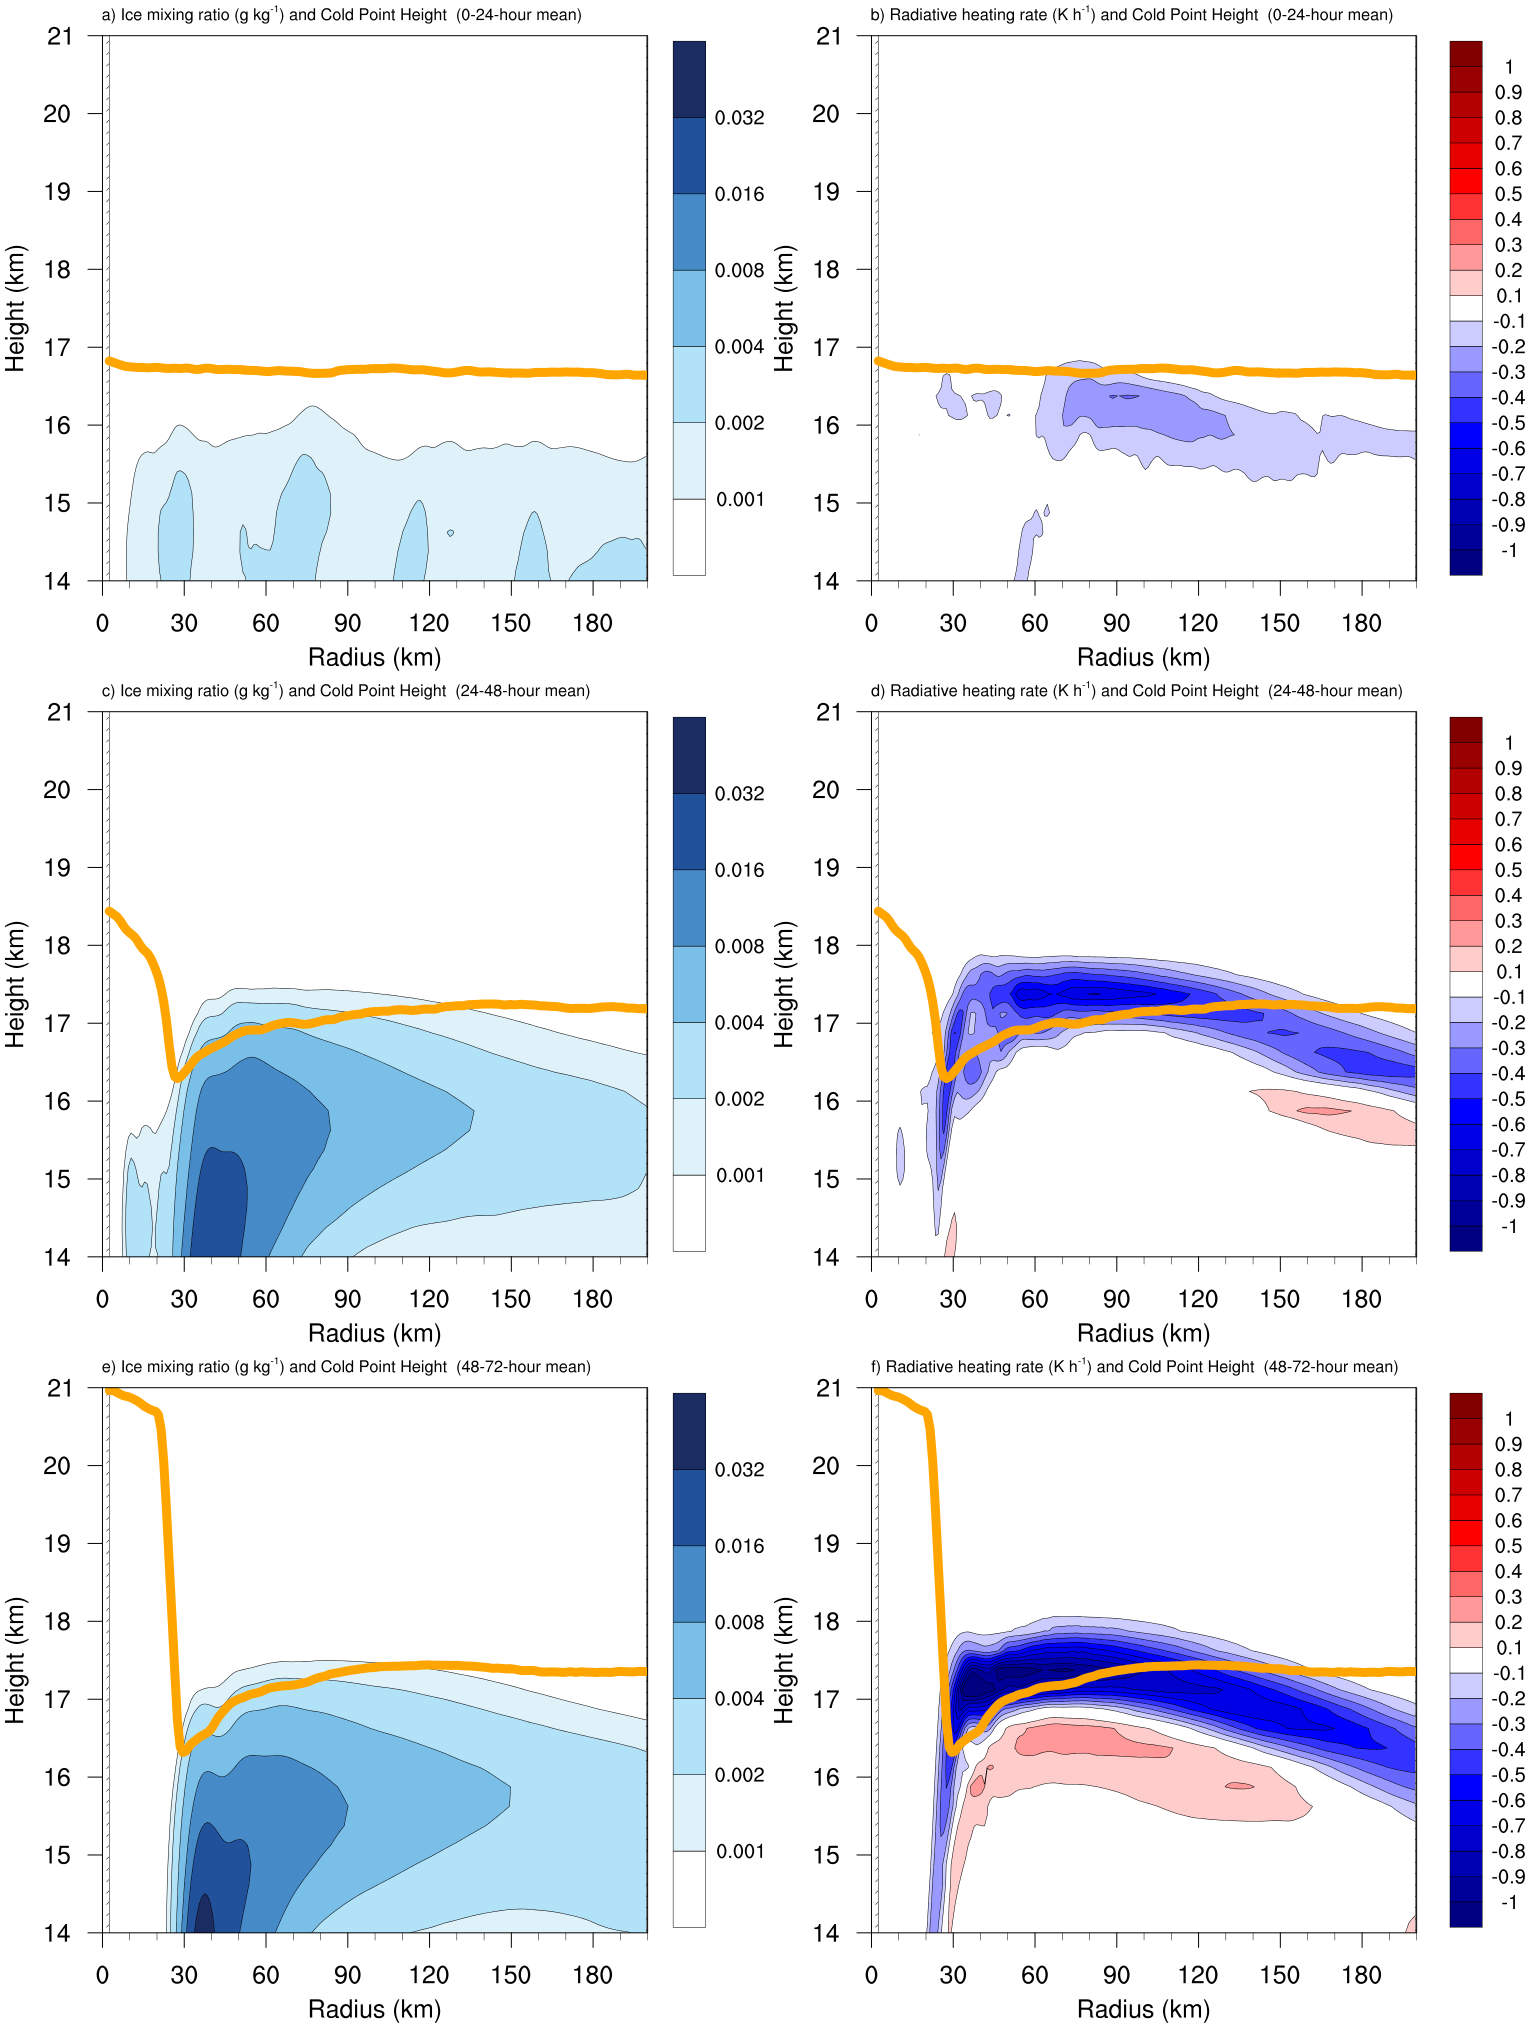
\includegraphics[width=39pc]{figures/qi+radten.png}}
\end{figure*}
\begin{figure}
\caption{Ice mixing ratio (g kg\textsuperscript{-1}) and cold-point tropopause height (orange lines) averaged over (a) 0-24 hours, (c) 24-48 hours, and (e) 48-72 hours. Radiative heating rate (K h\textsuperscript{-1}) and cold-point tropopause height (orange lines) averaged over (b) 0-24 hours, (d) 24-48 hours, and (f) 48-72 hours.} 
\label{fig:qi+radten}
\end{figure}

%FIGURE 10%
\begin{figure*}[ht]
\centerline{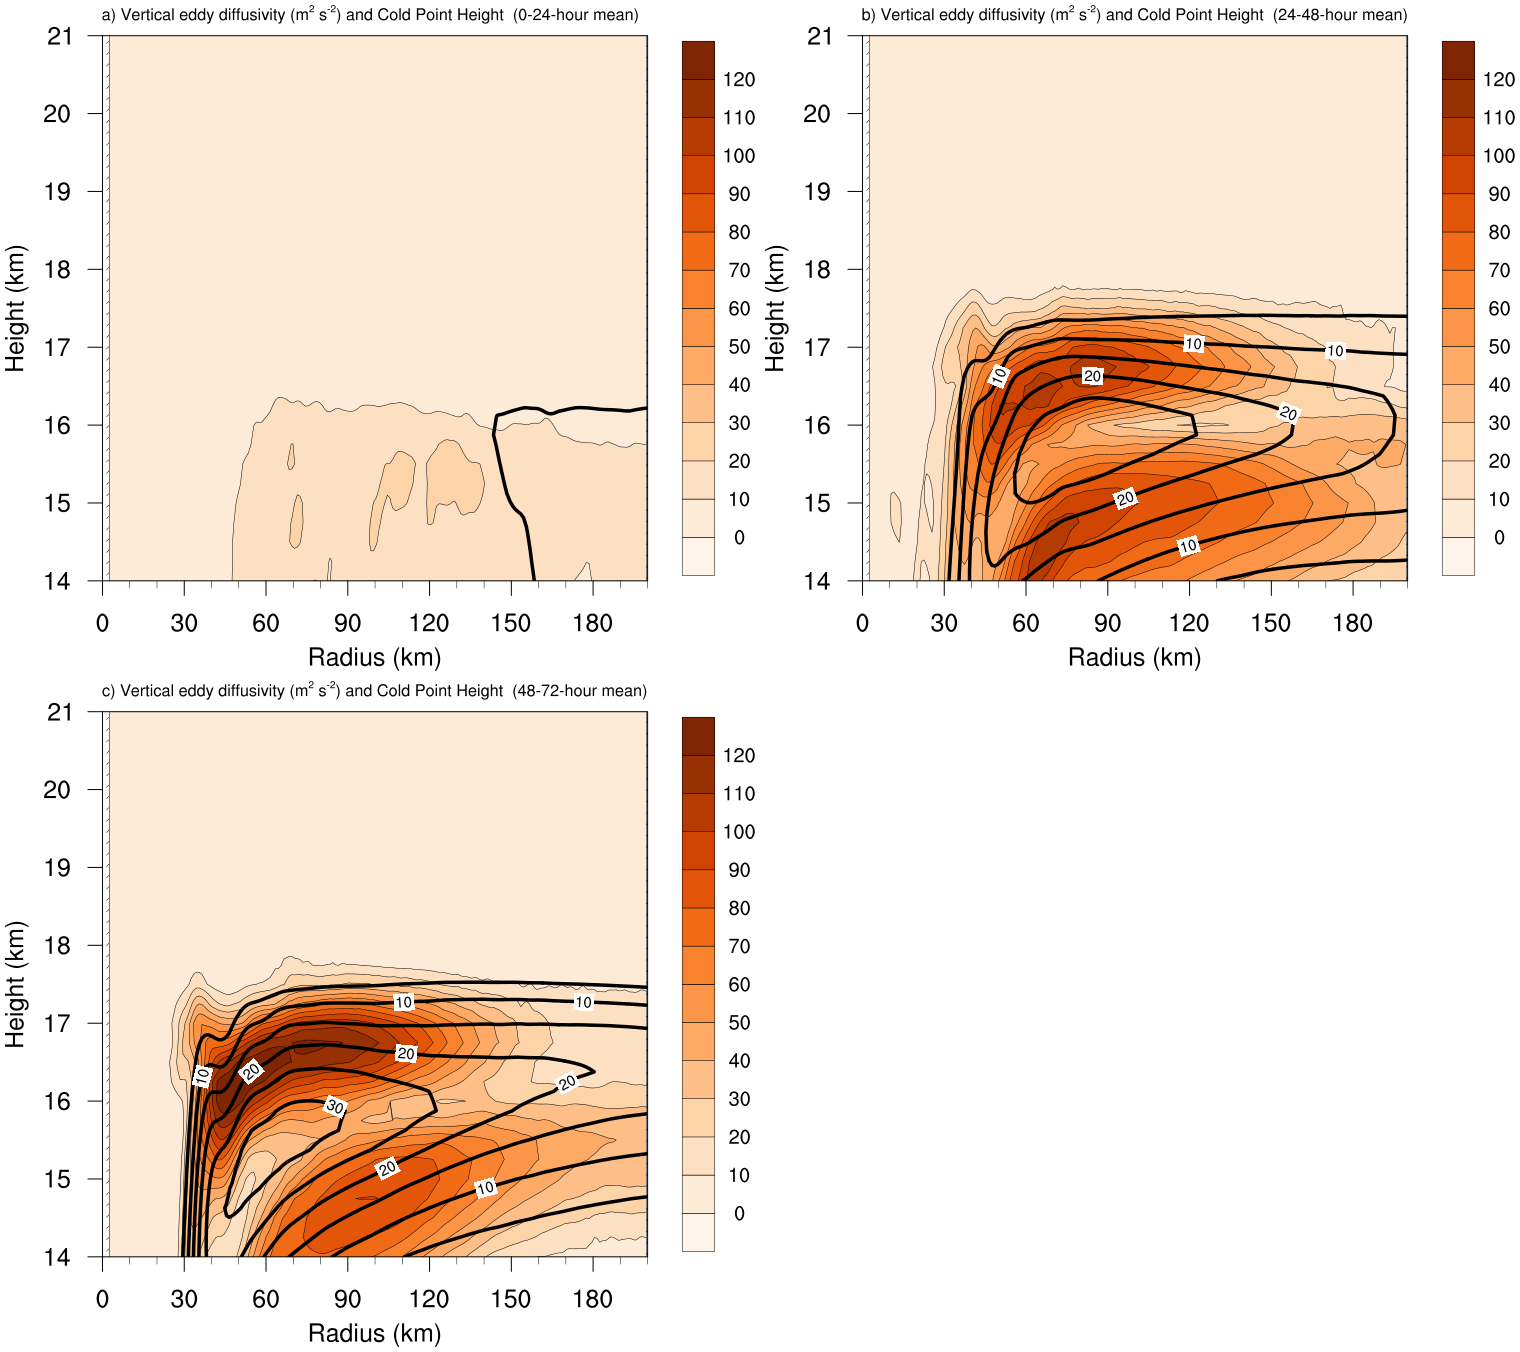
\includegraphics[width=39pc]{figures/khvten.png}}
\caption{Vertical eddy diffusivity (m\textsuperscript{2} s\textsuperscript{-2}; filled contours), cold-point tropopause height (cyan lines), and radial velocity (m s\textsuperscript{-1}; thick black lines) averaged over (a) 0-24 hours, (b) 24-48 hours, and (c) 48-72 hours.}
\label{fig:diff}
\end{figure*}

%FIGURE A1%
\begin{figure*}[ht]
\centerline{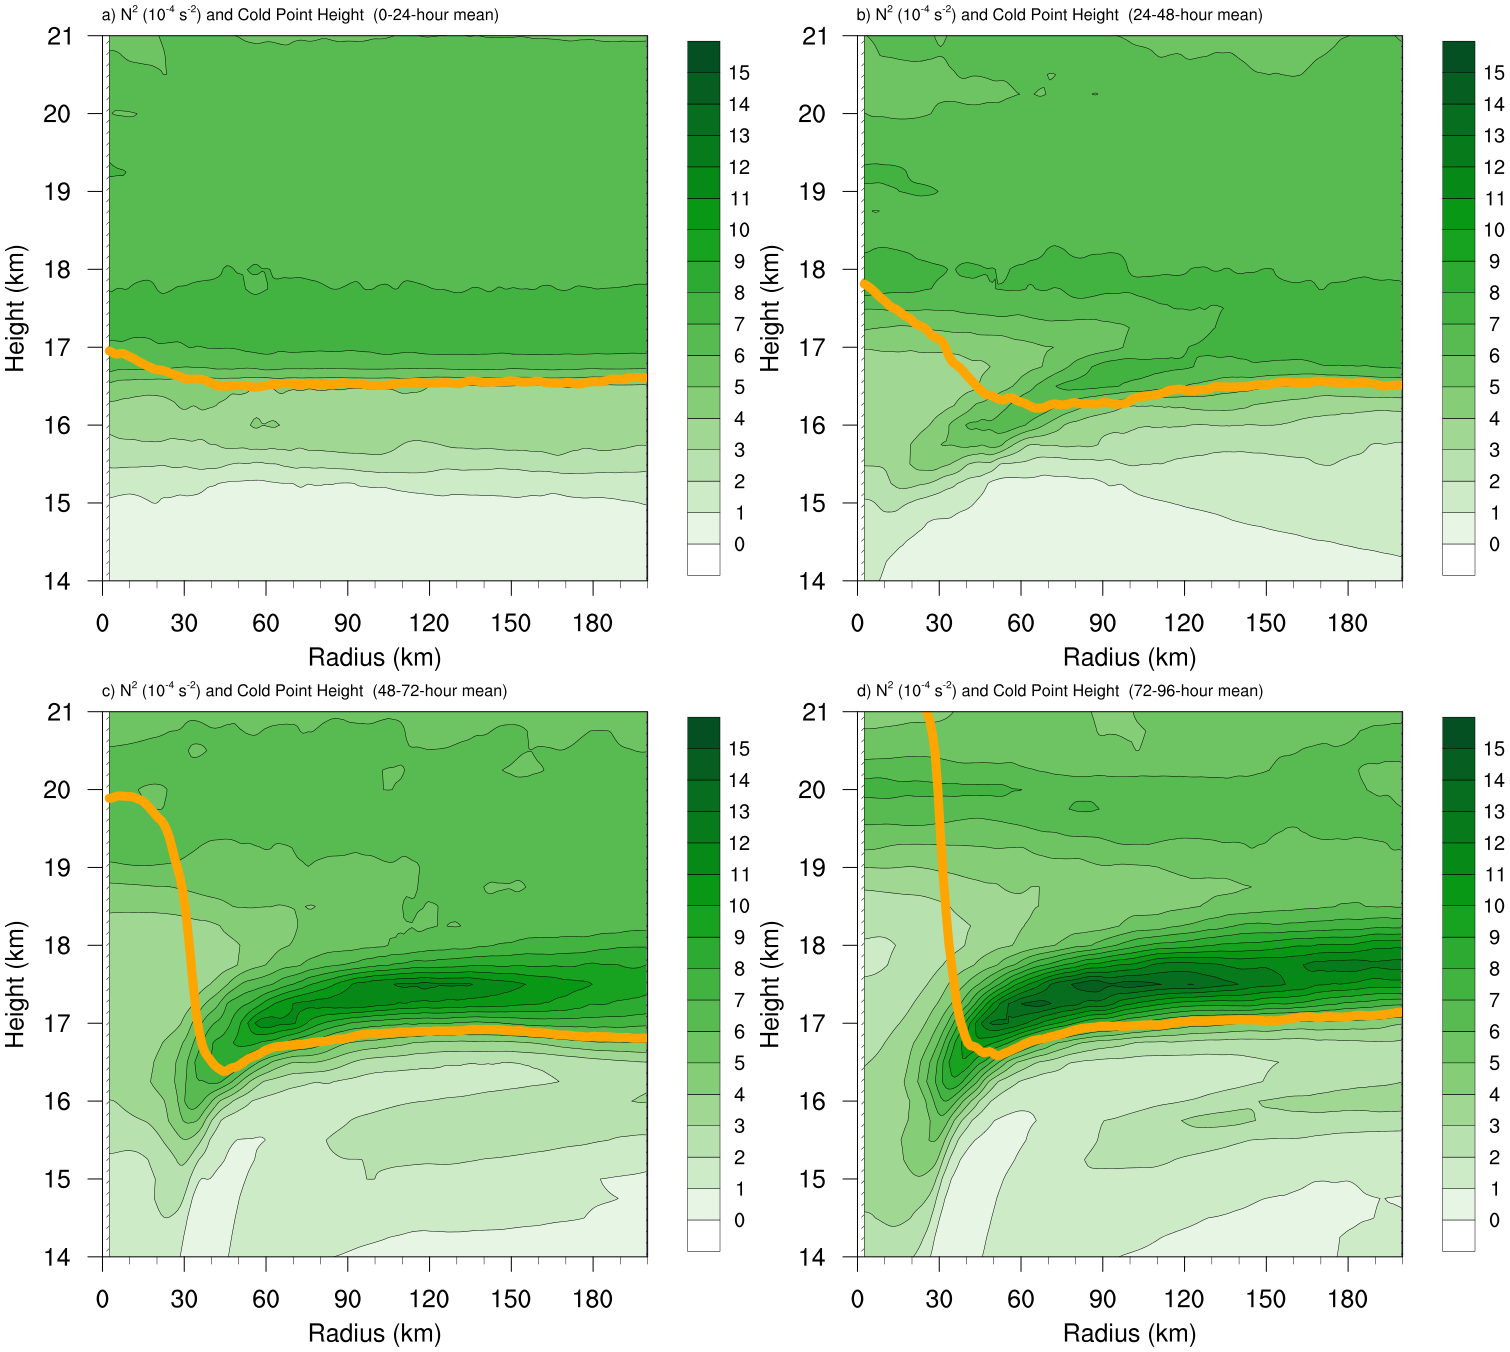
\includegraphics[width=39pc]{figures/n2-1000km.png}}
\appendcaption{A1}{Twenty-four-hour averages of squared Brunt-V{\"a}is{\"a}l{\"a} frequency ($N^2$; 10\textsuperscript{-4} s\textsuperscript{-2}) over (a) 0-24 hours, (b) 24-48 hours, (c) 48-72 hours, and (d) 72-96 hours for the simulation described in Appendix Aa. Orange lines represent the cold-point tropopause averged over the same time periods.}
\label{fig:n2-1000km}
\end{figure*}

%FIGURE A2%
\begin{figure*}[ht]
\centerline{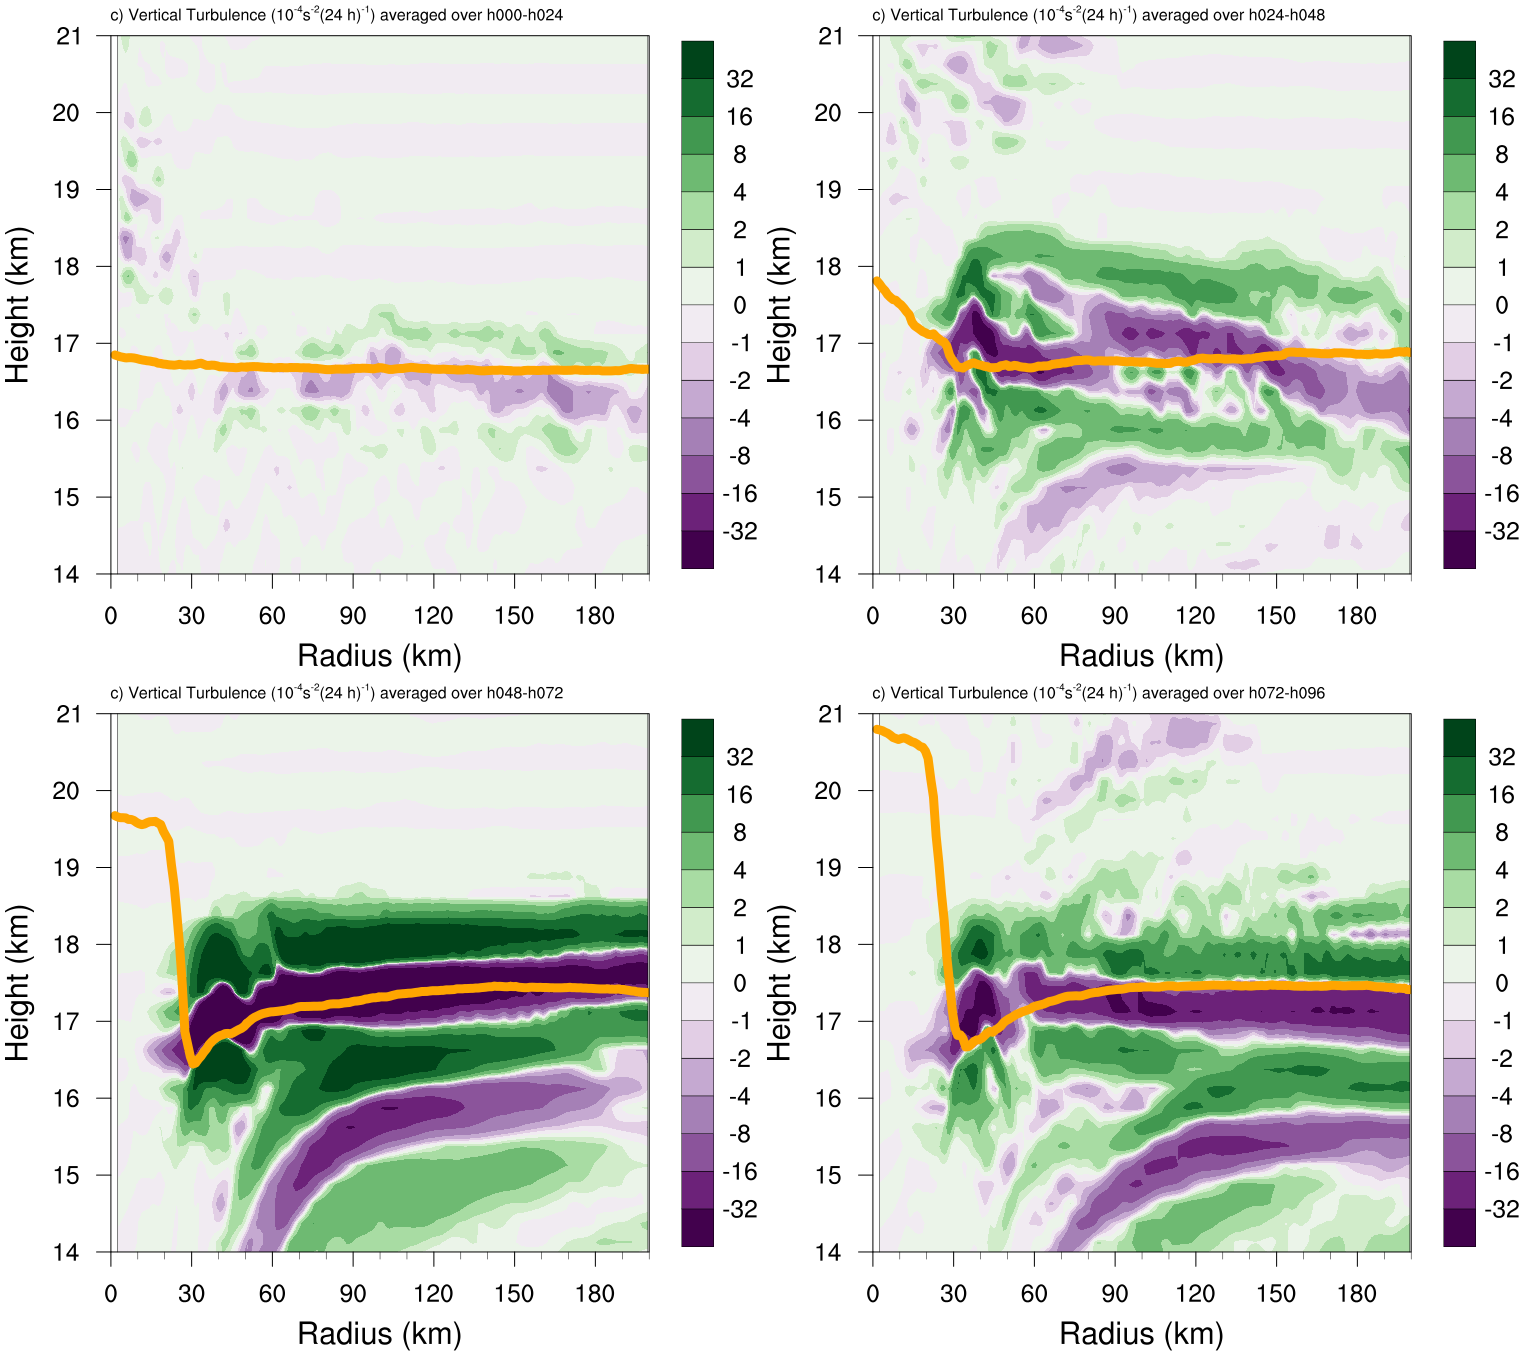
\includegraphics[width=39pc]{figures/turb-50m.png}}
\appendcaption{A2}{The contribution of vertical turbulence to the $N^2$ variability (10\textsuperscript{-4} s\textsuperscript{-2} (24 h)\textsuperscript{-1}) averaged over (a) 0-24 hours, (b) 24-48 hours, (c) 48-72 hours, and (d) 72-96 hours for the simulation described in Appendix Ab.}
\label{fig:turb-50m}
\end{figure*}

%\begin{figure}[t]
%\begin{figure}[t]
%\begin{figure}[t]
%  \noindent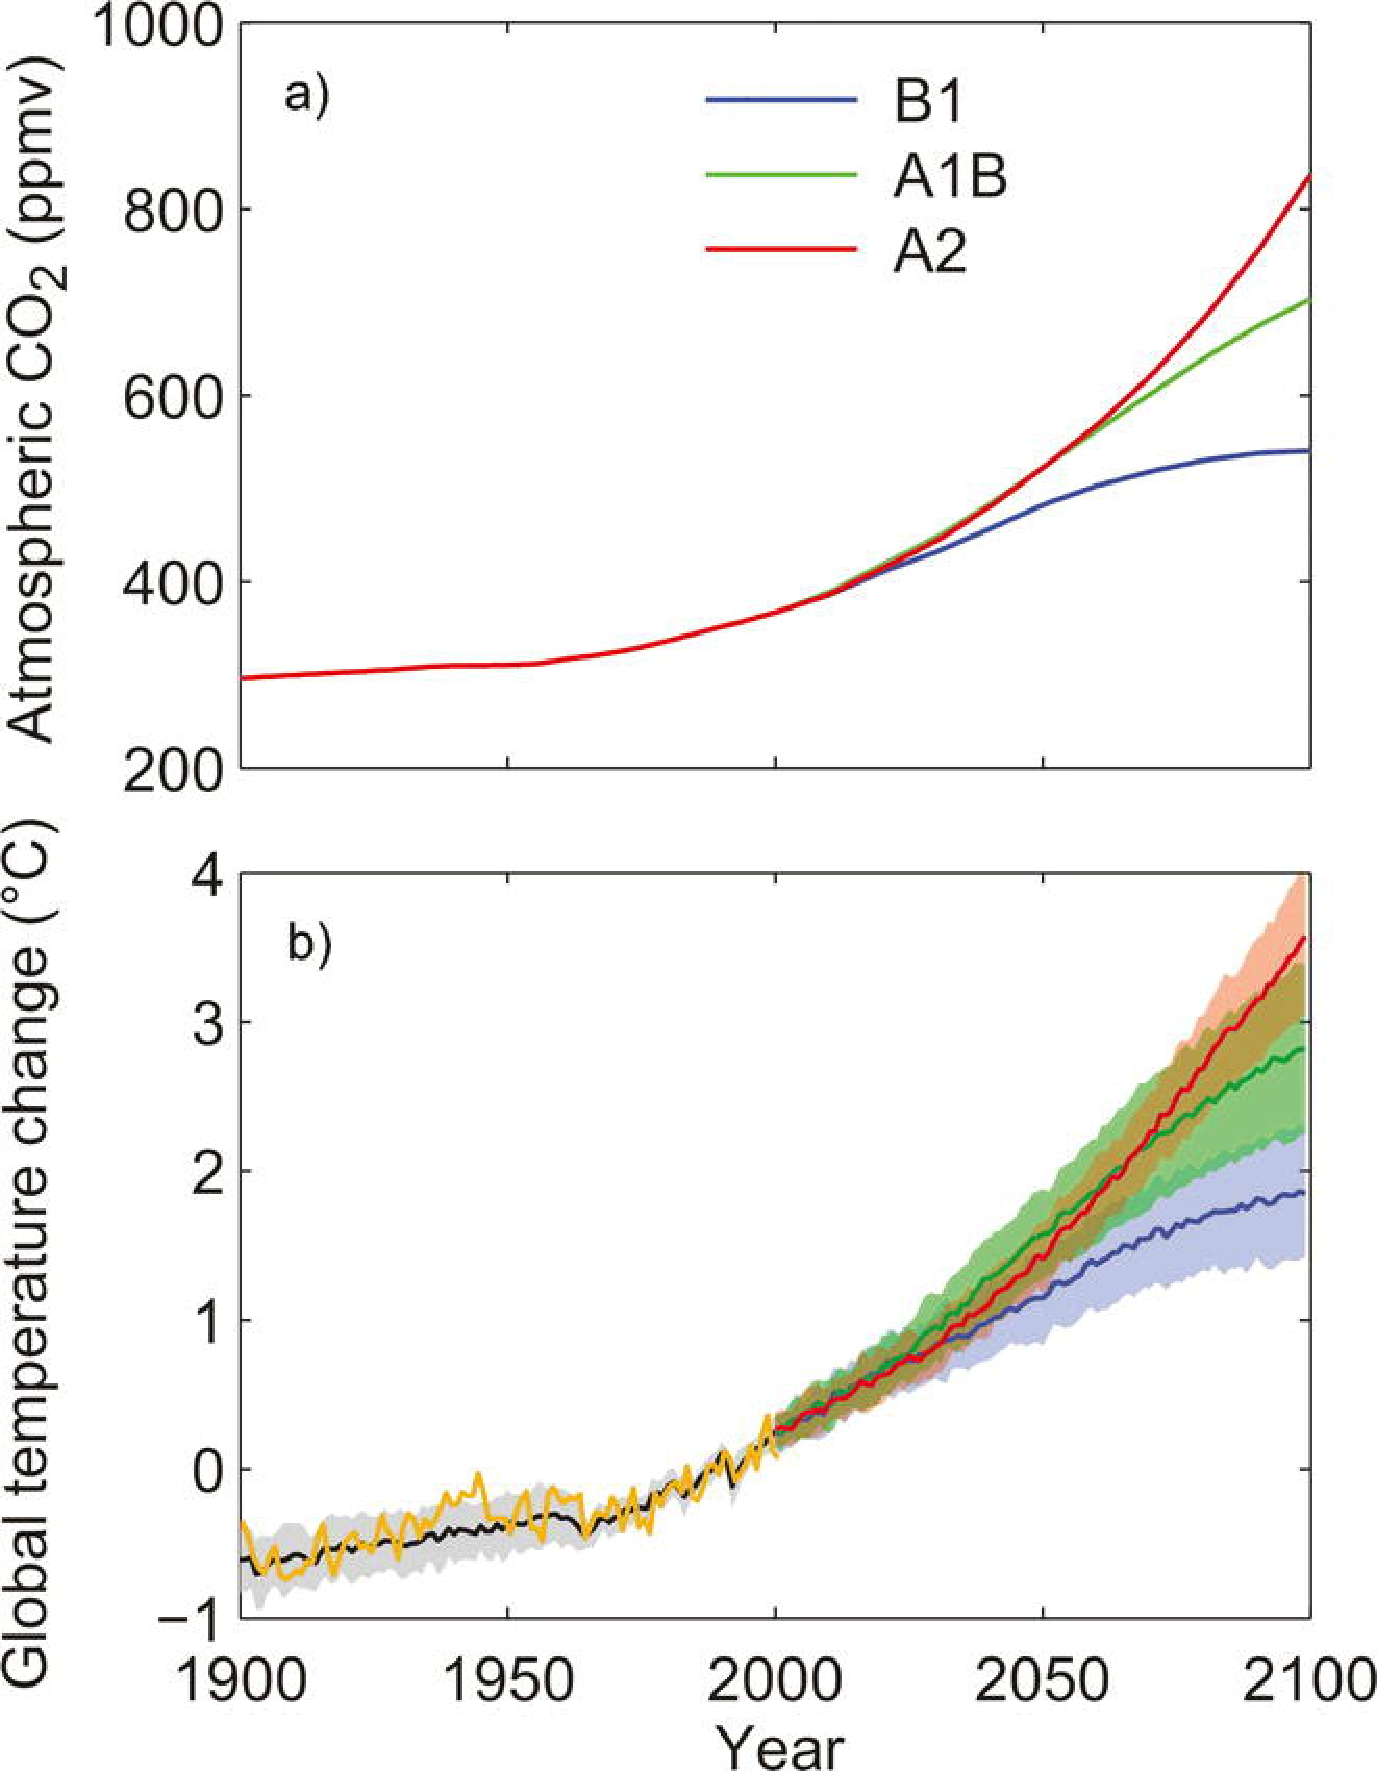
\includegraphics[width=19pc,angle=0]{figure01.pdf}\\
%  \caption{Enter the caption for your figure here.  Repeat as
%  necessary for each of your figures. Figure from \protect\cite{Knutti2008}.}\label{f1}
%\end{figure}

\end{document}
